\documentclass[dvipdfmx,a4paper,11pt]{article}
\usepackage[utf8]{inputenc}
%\usepackage[dvipdfmx]{hyperref} %リンクを有効にする
\usepackage{url} %同上
\usepackage{amsmath,amssymb} %もちろん
\usepackage{amsfonts,amsthm,mathtools} %もちろん
\usepackage{braket,physics} %あると便利なやつ
\usepackage{bm} %ラプラシアンで使った
\usepackage[top=30truemm,bottom=30truemm,left=25truemm,right=25truemm]{geometry} %余白設定
\usepackage{latexsym} %ごくたまに必要になる
\renewcommand{\kanjifamilydefault}{\gtdefault}
\usepackage{otf} %宗教上の理由でmin10が嫌いなので


\usepackage[all]{xy}
\usepackage{amsthm,amsmath,amssymb,comment}
\usepackage{amsmath}    % 数学用
\usepackage{amssymb}  
\usepackage{color}
\usepackage{amscd}
\usepackage{amsthm}  
\usepackage{wrapfig}
\usepackage{comment}	
\usepackage{graphicx}
\usepackage{setspace}
\usepackage{pxrubrica}
\usepackage{enumitem}
\usepackage{mathrsfs} 
\usepackage[colorlinks,linkcolor=red,anchorcolor=blue,citecolor=blue]{hyperref} 
\setstretch{1.2}
\usepackage{pgfplots}


\newcommand{\R}{\mathbb{R}}
\newcommand{\Z}{\mathbb{Z}}
\newcommand{\Q}{\mathbb{Q}} 
\newcommand{\N}{\mathbb{N}}
\newcommand{\C}{\mathbb{C}} 
\newcommand{\Sin}{\text{Sin}^{-1}} 
\newcommand{\Cos}{\text{Cos}^{-1}} 
\newcommand{\Tan}{\text{Tan}^{-1}} 
\newcommand{\invsin}{\text{Sin}^{-1}} 
\newcommand{\invcos}{\text{Cos}^{-1}} 
\newcommand{\invtan}{\text{Tan}^{-1}} 
\newcommand{\Area}{S}
\newcommand{\vol}{\text{Vol}}
\newcommand{\maru}[1]{\raise0.2ex\hbox{\textcircled{\tiny{#1}}}}
\newcommand{\sgn}{{\rm sgn}}
%\newcommand{\rank}{{\rm rank}}



   %当然のようにやる.
\allowdisplaybreaks[4]
   %もちろん.
%\title{第1回. 多変数の連続写像 (岩井雅崇, 2020/10/06)}
%\author{岩井雅崇}
%\date{2020/10/06}
%ここまで今回の記事関係ない
\usepackage{tcolorbox}
\tcbuselibrary{breakable, skins, theorems}

\theoremstyle{definition}
\newtheorem{thm}{定理}
\newtheorem{lem}[thm]{補題}
\newtheorem{prop}[thm]{命題}
\newtheorem{cor}[thm]{系}
\newtheorem{claim}[thm]{主張}
\newtheorem{dfn}[thm]{定義}
\newtheorem{rem}[thm]{注意}
\newtheorem{exa}[thm]{例}
\newtheorem{conj}[thm]{予想}
\newtheorem{prob}[thm]{問題}
\newtheorem{rema}[thm]{補足}
\newtheorem{dfnthm}[thm]{定義・定理}

\DeclareMathOperator{\Ric}{Ric}
\DeclareMathOperator{\Vol}{Vol}
 \newcommand{\pdrv}[2]{\frac{\partial #1}{\partial #2}}
 \newcommand{\drv}[2]{\frac{d #1}{d#2}}
  \newcommand{\ppdrv}[3]{\frac{\partial #1}{\partial #2 \partial #3}}
  
  \newcommand{\xb}[1]{\textcolor{blue}{#1}}
\newcommand{\xr}[1]{\textcolor{red}{#1}}
\newcommand{\xm}[1]{\textcolor{magenta}{#1}}


\title{2024年度春夏学期 \\ 大阪大学 全学共通教育科目 \\ 解析学入門 経(161〜) }
\author{岩井雅崇 (大阪大学)}
\date{\today \, ver 1.00}
%ここから本文.
\begin{document}

\maketitle
\tableofcontents
\newpage

\begin{center}
\setcounter{section}{-1}
\section{ガイダンス}
\label{sec-guide}
\end{center}

\begin{center}
{\Large 2024年度春夏学期 \\ 大阪大学 全学共通教育科目 解析学入門 経(161〜)} \\
木曜3限(13:30-15:00) 共B218
\end{center}
\begin{flushright}
 岩井雅崇(いわいまさたか) \\
\end{flushright}
{\Large \underline{基本的事項}}
\begin{itemize}
  \setlength{\parskip}{0cm} % 段落間
  \setlength{\itemsep}{0cm} % 項目間
\item この授業は\underline{対面授業}です. \underline{木曜3限(13:30-15:00)に共B218}にて授業を行います.
\item 授業ホームページ(\url{https://masataka123.github.io/2024_summer_calculus/})にて「授業の資料・授業の板書」などをアップロードしていきます. 
QRコードは下にあります.
\begin{figure}[htbp]
\begin{center}
 
\includegraphics[height=30mm, width=30mm]{calculus.png}
\end{center}
\end{figure}
\end{itemize}

\hspace{-18pt}{\Large \underline{成績に関して}}

\underline{演習(後述)と期末試験(後述)で成績をつける予定です. } 内訳は未定です. 単位が欲しい方はこの二つに必ず出席するようにしてください. 

なお通常時の授業(演習や期末試験以外の授業)に出席点はございません. そのため授業への出席は任意となります. 


\medskip
\hspace{-18pt}{\Large \underline{1. 演習に関して}}

次の日時に演習の授業を行います. 
\begin{itemize}
  \setlength{\parskip}{0cm} 
  \setlength{\itemsep}{0cm}
\item 日時: 2024年6月6日と2024年7月18日 木曜3限(13:30-15:00)
\item 場所: 共B218
\item 演習内容: 配布したプリントの問題を解いて提出してください. なお協力して解いても構いません. 
\end{itemize}
\underline{以上は予定であるため, 変更の可能性があります.} もし変更する場合はホームページやCLEで連絡します. 
なお代理出席などの行為は不正行為とみなし, 加担した人全員の単位を不可にします.
欠席する場合はあらかじめmasataka@math.sci.osaka-u.ac.jpにご連絡いただければ幸いです.\footnote{その場合は欠席理由をきちんとお伝えください. ただし正当な理由以外での欠席は認められません. (成績に関わるからです.) よくわからない場合はとりあえずメールしてください.}

\newpage
\hspace{-18pt}{\Large \underline{2. 期末試験に関して}}

現時点での期末試験の予定は次のとおりです. 
\begin{itemize}
  \setlength{\parskip}{0cm} 
  \setlength{\itemsep}{0cm}
\item 日時: 2024年 7月25日 木曜3限(13:30-15:00) (予定)
\item 場所: 共B218
\item 持ち込みに関して: A4用紙4枚(裏表使用可)まで持ち込み可. 工夫を凝らしてA4用紙4枚に今までの内容をまとめてください.
\item 試験内容 : 授業・演習でやった範囲
\end{itemize}
\underline{以上は予定であるため, 変更の可能性があります.} もし変更する場合はホームページやCLEで連絡します. 

\medskip
\hspace{-18pt}{\Large \underline{まとめ}}
\begin{enumerate}
  \setlength{\parskip}{0cm} 
  \setlength{\itemsep}{0cm} 
\item \underline{単位が欲しい方は演習に必ず出席し, 期末試験で成績が取れるくらいの点を取ってください.} 
\item 単位を認定するくらいの成績が取れていない場合, 容赦無く不可を出します. 
\item 講義への出席は自由です. 授業資料・授業の板書をホームページにアップロードするので, 自分の好きな方法で線形代数への理解を進めてください.\footnote{理由としては「私は講義をするのが上手くない」のと「もっと効率的な理解の方法があると思う」からです. この授業内容を理解するのに$1.5 \times 14 = 21$時間も本当にかかるのかと思います. (というか今の私は90分じっと講義を受けるのが好きではないです.  14週に分けて講義を聞くのも好きではないです. ) そして世の中には私よりもわかりやすい授業する人もいるので, そちらで理解を進めても良いと思います. 学び方は自由であり, その方法を制限するのは好きではありません. (つまり出席を取るのも好きではないです).}
\end{enumerate}


\vspace{11pt}
\hspace{-18pt}{\Large \underline{その他}}
\begin{itemize}
  \setlength{\parskip}{0cm} % 段落間
  \setlength{\itemsep}{0cm} % 項目間
  \item 休講情報は授業ホームページ・KOANでお知らせいたします.
  %\item 休講予定: 2024年1月18日 (休講はほぼ確定) 2023年11月28日または2023年11月30日 (どちらか休講にするかも・未確定). \footnote{他にも授業が早く終われば休講にします.} 
    %\item 演習問題と授業内容が噛み合ってない可能性があります.
  \item 休講情報や資料の修正などをするので, こまめにホームページを確認してください.
  \item 教科書は用いない. 参考書は「三宅敏恒著 入門線形代数」(培風館)を用いる.
   \item オフィスアワーを月曜16:00-17:00に設けています. この時間に私の研究室に来ても構いません(ただし来る場合は前もって連絡してくれると助かります.)
    %\item TAさんは演義の時間中に巡回しているので, 自由にご質問して構いません. 
    %\item $\pi$-base \url{https://topology.jdabbs.com}も活用してください. 
 \end{itemize}


\newpage 


\section{数列と極限}
\label{sec-1}
\subsection{記法}

\hspace{16pt}自然数などの記号

\begin{itemize}
  \setlength{\parskip}{0cm} 
  \setlength{\itemsep}{0cm}
\item $\N =\{ \text{自然数全体}\} = \{ 1,2,3,4,5,\cdots\}$
\item $\Z =\{ \text{整数全体}\} = \{ 0, \pm1, \pm 2,\cdots\}$
\item $\Q =\{ \text{有理数全体} \} = \left\{ \frac{m}{n} \,\,|\,\,  m,n \in \Z , n \neq 0 \right\}$
\item $\R =\{ \text{実数全体}\} $
\item $\R \setminus \Q=\{ x \in \R \,\, | \,\, x \not \in \Q\} = \{ \text{無理数全体}\} $
\end{itemize}

区間の表記

\begin{itemize}
  \setlength{\parskip}{0cm} 
  \setlength{\itemsep}{0cm}
\item $ [a,b] = \{ x \in \R \,\,| \,\, a \leqq x \leqq b\}$ ($a,b$ 共に実数)
\item $ [a,b) = \{ x \in \R \,\,| \,\, a \leqq x < b\}$ ($a$は実数, $b$は実数または$+\infty$)\footnote{$+ \infty$は実数ではないが限りなく大きなものとして扱います. 一種の記法です. $- \infty$も同様に限りなく小さいものとして扱います.}
\item $ (a,b] = \{ x \in \R \,\,| \,\, a < x \leqq b\}$ ($a$は実数または$-\infty$, $b$は実数)
\item $ (a,b) = \{ x \in \R \,\,| \,\, a < x < b\}$ ($a$は実数または$-\infty$, $b$は実数または$+\infty$)
\end{itemize}

特に\underline{$(a,b)$を開区間}といい, \underline{$ [a,b]$を閉区間}という.
この記法により, $\R = (- \infty, + \infty)$である.

\subsection{数列の極限・ネイピア数}
 \begin{tcolorbox}[
    colback = white,
    colframe = green!35!black,
    fonttitle = \bfseries,
    breakable = true]
    \begin{dfn}[数列の極限の感覚的な定義]
\underline{数列が$\{a_n\}_{n=1}^{\infty}$が極限$\alpha \in \R$を持つ}とは, $n$を大きくしていくと$a_n$が$\alpha$に限りなく近づくこと.
このとき
$$
\lim_{n \rightarrow \infty} a_n = \alpha \text{\,\,または\,\,} 
a_n \xrightarrow[n \rightarrow \infty]{} \alpha 
$$
とかき, \underline{$a_n$は$\alpha$に収束する}という.
$a_n$が収束しないとき, \underline{$a_n$は発散する}という.

\hspace{12pt}%数列が$\{a_n\}_{n=1}^{\infty}$が
$n$を大きくしていくと, $a_n$が限りなく大きくなるとき, \underline{$\lim_{n \rightarrow \infty} a_n =+\infty $と書く.}
限りなく小さくなるとき, \underline{$\lim_{n \rightarrow \infty} a_n   = - \infty $と書く.}
 \end{dfn}
 \end{tcolorbox}
 
 \begin{exa}
 \begin{itemize}
   \setlength{\parskip}{0cm} 
  \setlength{\itemsep}{0cm}
\item $a_n = \frac{1}{n}$からなる数列は$n$を大きくしていくと0に収束する. よって$\lim_{n \to \infty}a_n =0$である. \footnote{今回極限の定義を感覚的なものにしているため, この事柄は証明することはできない. 極限はもっと厳密に$\epsilon$-$N$論法というものを用いて定義される(が非常にわかりづらい...)}
\item $a_n = n$からなる数列は, $n$を大きくしていくと, $a_n$が限りなく大きくなる. よって$a_n$は発散する. $\lim_{n \to \infty}a_n =+\infty$である. 

\item $a_n = (-1)^{n}$からなる数列は発散する. 

\end{itemize}
\end{exa}

\begin{exa}
$A$を正の実数とし, $a_n = A^{n}$とする.
このとき収束発散は次の通りになる.
 \begin{itemize}
   \setlength{\parskip}{0cm} 
  \setlength{\itemsep}{0cm}
\item $A<1$のとき$a_n$は$n$を大きくしていくと0に収束する.
\item $A=1$のとき$a_n$は$n$を大きくしていくと1に収束する.
\item $A>1$のとき$a_n$は$n$を大きくしていくと$+\infty$に発散する.
 \end{itemize}
\end{exa}




  \begin{tcolorbox}[
    colback = white,
    colframe = green!35!black,
    fonttitle = \bfseries,
    breakable = true]
    \begin{thm}
数列$\{ a_n \}$と$\alpha \in \R$について, 
$\lim_{n \rightarrow \infty } | a_n - \alpha |  = 0$ならば
$\lim_{n \rightarrow \infty }a_n =\alpha$である.
 \end{thm}
 \end{tcolorbox}

  \begin{tcolorbox}[
    colback = white,
    colframe = green!35!black,
    fonttitle = \bfseries,
    breakable = true]
    \begin{thm}[はさみうちの原理.]
$\alpha \in \R$と$a_n \leqq b_n \leqq c_n$となる数列$\{ a_n \}$, $\{ b_n \}$, $\{ c_n \}$
に関して次が成り立つ.
\begin{enumerate}
  \setlength{\parskip}{0cm} 
  \setlength{\itemsep}{0cm}
\item $\lim_{n \rightarrow \infty }a_n = \lim_{n \rightarrow \infty }c_n =\alpha$
ならば
$\lim_{n \rightarrow \infty }b_n =\alpha$である.
\item $\lim_{n \rightarrow \infty }a_n = +\infty$
ならば
$\lim_{n \rightarrow \infty }b_n =+\infty$である.
\item $\lim_{n \rightarrow \infty }c_n = -\infty$
ならば
$\lim_{n \rightarrow \infty }b_n =-\infty$である.
\end{enumerate}
 \end{thm}
 \end{tcolorbox}
 
 
  
   \begin{tcolorbox}[
    colback = white,
    colframe = green!35!black,
    fonttitle = \bfseries,
    breakable = true]
    \begin{prop}[極限の性質]
    \label{prop-limit}
 
  $\alpha, \beta, c \in \R$とする.  $\lim_{n \rightarrow \infty} a_n = \alpha$, 
    $\lim_{n \rightarrow \infty} b_n = \beta$であるとき, 以下が成り立つ.
 \begin{itemize}
   \setlength{\parskip}{0cm} 
  \setlength{\itemsep}{0cm}
 \item $\lim_{n \rightarrow \infty} (a_n \pm b_n) = \alpha \pm \beta$.
  \item $\lim_{n \rightarrow \infty} (c a_n ) = c\alpha $.
   \item $\lim_{n \rightarrow \infty} (a_n b_n) = \alpha  \beta$.
    \item $\lim_{n \rightarrow \infty} \frac{a_n}{b_n} = \frac{\alpha}{\beta}$.
    ($\beta \neq 0$のとき.)
 \end{itemize}
        \end{prop}
 \end{tcolorbox}
 
  \begin{exa}
 $a_n = \sum_{k=1}^{n}\frac{1}{k(k+1)}$からなる数列は$n$を大きくしていくと1に収束する. よって$\lim_{n \to \infty}a_n =1$である.
\end{exa}

   \begin{exa}
  命題 \ref{prop-limit}は発散する場合(つまり$\alpha$, $\beta$が$\infty$や$- \infty$となる場合)には成り立たない. 
実際$a_n = n$, $b_n=-n$とすると$\lim_{n \to \infty}a_n=+ \infty$, $\lim_{n \to \infty}b_n=- \infty$だが$\lim_{n \to \infty} \left(a_n + b_n\right) =0$である.
\footnote{$a_n = n^2$, $b_n=-n$のときは$\lim_{n \to \infty} \left(a_n + b_n\right) = + \infty$となる. つまり\underline{$\infty$を数と同様に扱ってはいけない!}}
\end{exa}



  \begin{exa}
  \label{exa-frac}
$a$を正の実数とするとき,  $\lim_{n \to + \infty}\frac{a^n}{n!} =0$.
  \end{exa}
 


 \begin{tcolorbox}[
    colback = white,
    colframe = green!35!black,
    fonttitle = \bfseries,
    breakable = true]
    \begin{thm}[実数の連続性]
    \label{realconti}
$\R$の数列$\{ a_n \}$が次の2つを満たすとする. 
 \begin{itemize}
   \setlength{\parskip}{0cm} 
  \setlength{\itemsep}{0cm}
  \item ある実数$M$があって任意の$n$について$a_n \leqq M$(上に有界).
  \item 任意の$n$について$a_n \leqq a_{n+1}$(単調増加).
  \end{itemize}
  このとき数列$\{ a_n \}$はある値$\alpha \in \R$に収束する.
 \end{thm}
  \end{tcolorbox}
  
    
  \begin{tcolorbox}[
    colback = white,
    colframe = green!35!black,
    fonttitle = \bfseries,
    breakable = true]
 \begin{thm}[ネイピア数]
 $$
 \lim_{n \to \infty} \left( 1 + \frac{1}{n}\right)^{n}
 $$
 は収束する. その値を$e$とかき\underline{ネイピア数}と呼ぶ.
  \end{thm}
   \end{tcolorbox}
ネイピア数は無理数であることが知られている. 
\subsection{関数と極限}

%以下この授業を通してよく使う記号や用語をまとめる.(興味がなければ飛ばして良い)

%\subsection{関数}

 \begin{tcolorbox}[
    colback = white,
    colframe = green!35!black,
    fonttitle = \bfseries,
    breakable = true]
    \begin{dfn}[]
 $A$を$\R$の部分集合とする.
 任意の$x \in A$について, 実数$f(x)$がただ一つ定まるとき, 
 \underline{$f(x)$を$A$上の関数}といい
    $$
\begin{array}{cccc}
f: &A& \rightarrow & \R  \\
&x& \longmapsto & f(x)
\end{array}
\text{\,\,と書く.}
$$
\end{dfn}

また
$$
\{(x,y) \in \R^2 \,|\, y=f(x)\}
$$
を関数$y=f(x)$のグラフという.
  \end{tcolorbox}
 %以下$f(A) = \{ f(x) \,\,|\,\, x \in A\}$とする.

\begin{exa}
 $$
\begin{array}{cccc}
f: &\R& \rightarrow & \R  \\
&x& \longmapsto & x^2
\end{array}
$$
は$\R$上の関数. 
関数$y=f(x)$のグラフは2次関数のグラフである. 
\end{exa}

\begin{exa}
\label{exa-disconti}
     $$
\begin{array}{cccc}
f: &\R& \rightarrow & \R  \\
&x& \longmapsto & 
\begin{cases}
    1& (x >0) \\
    0& (x \le 0)
  \end{cases}
\end{array}
$$
は$\R$上の関数である. 
\end{exa}


 \begin{tcolorbox}[
    colback = white,
    colframe = green!35!black,
    fonttitle = \bfseries,
    breakable = true]
    \begin{dfn}[関数の極限]
$a\in \R$とし$f(x)$を$a$の周りで定義された関数とする.
$x \rightarrow a$のとき, \underline{$f(x)$が$\alpha \in \R$に収束する}とは
$x \neq \alpha$を満たしながら$x$を$a$に近づけるとき, $f(x)$が限りなく$\alpha$に近づくこと.
このとき
$$
\lim_{x \rightarrow a} f(x) = \alpha \text{\,\,または\,\,}
f(x) \xrightarrow[x \rightarrow a]{} \alpha 
\text{\,\,と書く.}
$$

 また数列のときと同様に
 $\lim_{x \rightarrow a} f(x) = \pm\infty$や
  $\lim_{x \rightarrow \pm \infty} f(x) = \alpha$などを定める. 
\end{dfn}
  \end{tcolorbox}


  

  
  \begin{exa}
     $$
\begin{array}{cccc}
f: &[-1,1]& \rightarrow & \R  \\
&x& \longmapsto & x^2
\end{array}
$$
について, $\lim_{x \rightarrow 0} f(x) =0.$
\end{exa}

  \begin{exa}
     $$
\begin{array}{cccc}
f: &(0 , +\infty)& \rightarrow & \R  \\
&x& \longmapsto & \frac{1}{x}
\end{array}
$$
について, $\lim_{x \rightarrow +\infty} f(x) =0$である.
\end{exa}

数列のときと同様に次が成り立つ. 
  \begin{tcolorbox}[
    colback = white,
    colframe = green!35!black,
    fonttitle = \bfseries,
    breakable = true]
    \begin{thm}
$a\in \R$とし$f(x)$を$a$の周りで定義された関数と$\alpha \in \R$について, 
$\lim_{x \rightarrow a } | f(x) - \alpha |  = 0$ならば
$\lim_{x \rightarrow a } f(x) =\alpha$である.
 \end{thm}
 \end{tcolorbox}

  \begin{tcolorbox}[
    colback = white,
    colframe = green!35!black,
    fonttitle = \bfseries,
    breakable = true]
    \begin{thm}
   $a\in \R$とし$f(x), g(x), h(x)$を$a$の周りで定義された関数で$f(x) \leqq g(x) \leqq h(x)$となるものに関して, $\lim_{x \rightarrow a}f(x)= \lim_{x \rightarrow a }h(x) =\alpha$
ならば$\lim_{x \rightarrow a} g(x) =\alpha$である.

 \end{thm}
 \end{tcolorbox}
 

 \begin{tcolorbox}[
    colback = white,
    colframe = green!35!black,
    fonttitle = \bfseries,
    breakable = true]
    \begin{prop}[極限の性質]
     $a$を実数または$\pm \infty$とし, $\alpha, \beta, c \in \R$とする. 
  $\lim_{x \rightarrow a} f(x) = \alpha$, 
    $\lim_{x \rightarrow a} g(x)= \beta$であるとき, 以下が成り立つ.
 \begin{itemize}
   \setlength{\parskip}{0cm} 
  \setlength{\itemsep}{0cm}
 \item $\lim_{x \rightarrow a}  (f(x) \pm g(x)) = \alpha \pm \beta$.
  \item $\lim_{x \rightarrow a} (c f(x)) = c\alpha $.
   \item $\lim_{x \rightarrow a}  (f(x)g(x)) = \alpha  \beta$.
    \item $\lim_{x \rightarrow a} \frac{f(x)}{g(x)} = \frac{\alpha}{\beta}$.
    ($\beta \neq 0$のとき.)
 \end{itemize}
 \end{prop}
   \end{tcolorbox}
   
数列のときと同様, 上の命題は$\alpha$, $\beta$が$\infty$や$- \infty$となる場合には成り立つとは限らない. 

  \begin{tcolorbox}[
    colback = white,
    colframe = green!35!black,
    fonttitle = \bfseries,
    breakable = true]
    \begin{prop}
$$
\lim_{x \rightarrow 0} \frac{\sin x}{x} =1
$$
 \end{prop}
 \end{tcolorbox}

\subsection{関数の連続性}
 
  \begin{tcolorbox}[
    colback = white,
    colframe = green!35!black,
    fonttitle = \bfseries,
    breakable = true]
    \begin{dfn}[連続の定義]
$a\in \R$とし$f(x)$を$a$の周りで定義された関数とする. \\
\underline{$f(x)$が$x=a$で連続}とは, 
$$
\lim_{x \rightarrow a } f(x) = f(a) 
\text{\,\,となること.}
$$
$f(x)$を区間$I$上の関数とする. \underline{$f(x)$が$I$上で連続}とは, 
任意の$a \in I$に関して$f(x)$が$a$で連続となること.
\end{dfn}
  \end{tcolorbox}

\begin{exa}
$\sin  x$や$\cos x$は$\R$上の連続関数
\end{exa}

  
   \begin{exa}
 例\ref{exa-disconti}での$f(x)$は$x=0$で連続ではない.
   \end{exa}

 
  \begin{tcolorbox}[
    colback = white,
    colframe = green!35!black,
    fonttitle = \bfseries,
    breakable = true]
    \begin{prop}
  $f(x), g(x)$共に$x=a$で連続ならば, $f(x) \pm g(x)$, $c f(x)$,  $f(x)g(x)$, $\frac{f(x)}{g(x)} $(ただし$g(a) \neq 0$)などは$x=a$で連続.
 \end{prop}
   \end{tcolorbox}

  \begin{tcolorbox}[
    colback = white,
    colframe = green!35!black,
    fonttitle = \bfseries,
    breakable = true]
    \begin{prop}
  $y=f(x)$が$x=a$で連続であり, $z=g(y)$が$y=f(a)$で連続ならば, 
  $z=g(f(x))$は$x=a$で連続.
 \end{prop}
   \end{tcolorbox}
   

   よって上の命題から, みんながよく知っている関数は(だいたい)連続関数. つまり$x^2, \tan x, \frac{1}{x^2 +1}$などは連続関数である. 


   \begin{tcolorbox}[
    colback = white,
    colframe = green!35!black,
    fonttitle = \bfseries,
    breakable = true]
    \begin{thm}[最大最小の存在定理]
$f(x)$が閉区間$[a,b]$上で連続ならば, $f(x)$は$[a,b]$上で最大値, 最小値を持つ.
 \end{thm}
   \end{tcolorbox}

 
    \begin{tcolorbox}[
    colback = white,
    colframe = green!35!black,
    fonttitle = \bfseries,
    breakable = true]
    \begin{thm}[中間値の定理]
$f(x)$を閉区間$[a,b]$上の連続関数とする.
$f(a) < f(b)$ならば, 任意の$\alpha \in [f(a), f(b)]$について, ある$c \in [a,b]$があって$f(c) = \alpha$となる.
 \end{thm}
   \end{tcolorbox}
   
 \subsection{指数関数・対数関数・無理関数}


   
   
\begin{tcolorbox}[
    colback = white,
    colframe = green!35!black,
    fonttitle = \bfseries,
    breakable = true]
    \begin{dfn}[指数関数・対数関数]
    \text{}
 \begin{itemize}
\item $a>0$かつ$a \neq 1$なる実数$a$について, 関数
$$
\begin{array}{cccc}
a^x: &\R& \rightarrow & (0, + \infty)  \\
&x& \longmapsto & a^x
\end{array}
$$
を\underline{指数関数}と呼ぶ.
$a=e$のとき, $e^x$を$\exp x$ともかく.

\item  $a>0$かつ$a \neq 1$なる実数$a$について, $\log_{a} x$を$a^{y}=x$となるただ一つの$y$として定める. ($a_x$の逆関数ともいう.)
この関数
$$
\begin{array}{cccc}
\log_{a} x: &(0, + \infty) & \rightarrow & \R \\
&x& \longmapsto & \log_{a} x
\end{array}
$$
を\underline{対数関数}と呼ぶ.
$a=e$のとき, $\log x$と書く.
 \end{itemize}
 \end{dfn}
   \end{tcolorbox}
   $a^{x}$, $\log_{a} x$ともに連続関数であることが知られている. 
   
   \begin{tcolorbox}[
    colback = white,
    colframe = green!35!black,
    fonttitle = \bfseries,
    breakable = true]
    \begin{lem}
    \text{}
    \begin{itemize}
      \setlength{\parskip}{0cm} 
  \setlength{\itemsep}{0cm}
  \item (底の変換公式) $\log_{a}x = \frac{\log x}{\log a}$,  $a^{x} = e^{(\log a)x}$.
  \item $\lim_{x \to +\infty}\frac{\log x}{x}=0$, $\lim_{x \to +\infty}\frac{x}{e^x}=0$.
\item $\lim_{x \to 0}\frac{\log(1+x)}{x} = 1, \lim_{x \to 0}\frac{e^x - 1}{x} =1$.
\end{itemize}
 \end{lem}
   \end{tcolorbox}
   
      よって指数関数・対数関数はネイピア数$e$のみ考えれば良い. 
      
   
 
 \begin{tcolorbox}[
    colback = white,
    colframe = green!35!black,
    fonttitle = \bfseries,
    breakable = true]
    \begin{dfn}[無理関数]
実数$\alpha$について$x^{\alpha}$を
$$
\begin{array}{cccc}
x^{\alpha}: &(0, + \infty) & \rightarrow & \R \\
&x& \longmapsto & x^{\alpha}:= e^{\alpha (\log x)}
\end{array}
$$
として定義し, \underline{無理関数}と呼ぶ. 
これは連続関数になる. 
  \end{dfn}
   \end{tcolorbox}
   
\begin{tcolorbox}[
    colback = white,
    colframe = green!35!black,
    fonttitle = \bfseries,
    breakable = true]
    \begin{lem}
$n$を1以上の自然数とする.
            \begin{itemize}
      \setlength{\parskip}{0cm} 
  \setlength{\itemsep}{0cm}
  \item  $x^{n}$は$x$の$n$乗であり, $x^{-n} = \frac{1}{x^n}$である. 
  \item $(x^{\frac{1}{n}})^n=x$. 特に$x^{\frac{1}{2}}=\sqrt{x}$である. 
\end{itemize}
 \end{lem}
   \end{tcolorbox}
つまり無理関数は多項式や平方根を拡張した概念である.  

\section{1変数の微分 -1階微分-}
\subsection{微分の定義・図形的な意味}
\begin{tcolorbox}[
    colback = white,
    colframe = green!35!black,
    fonttitle = \bfseries,
    breakable = true]
    \begin{dfn}
 $f(x)$を点$a$を含む開区間上の関数とする.
 \underline{$f(x)$が$x=a$で微分可能}とは
    $$ \lim_{x \rightarrow a} \frac{f(x) - f(a)}{x-a} \text{\,\,が存在すること.\,\,} $$
    この値を$f'(a)$と書く.
    $f'(a)$は$\drv{f}{x}|_{x=a}$や$\drv{f(a)}{x}$とも書く.
    
 \hspace{12pt}\underline{$f(x)$が$I$上で微分可能}とは, 任意の$a \in I$に関して
 $f(x)$が$x=a$で微分可能であること. このとき
  $$
\begin{array}{cccc}
f': &I& \rightarrow & \R  \\
&x& \longmapsto & f'(x)
\end{array}
$$
を\underline{$f(x)$の導関数}という. $f'(x)$は$\drv{f}{x}$とも書く.
    \end{dfn}
\end{tcolorbox}


   \begin{exa}
$n$を1以上の自然数とし, $f(x) = x^n$とする.
$f'(x) = n x^{n-1}$である. 
   \end{exa}

   
   
   
   \begin{exa}
   みんながよく知っている関数は(だいたい)微分可能関数. つまり$x^2,\sin x, \cos x, e^x $などは微分可能な関数である. 
   また$f(x)$が$x=a$で微分可能ならば$x=a$で連続である.
   \end{exa}

   
    \begin{tcolorbox}[
    colback = white,
    colframe = green!35!black,
    fonttitle = \bfseries,
    breakable = true]
    \begin{thm}
微分可能な関数$f(x)$について, 点$(a, f(a))$での接線の方程式は
$
y - f(a) = f'(a) (x-a) 
$
である.
\end{thm}
  \end{tcolorbox}
 
 \begin{exa}
 $f(x) = x^2 -1$の点$(1,0)$での接線の方程式は, $f'(x)=2x$であるので
 $y  = f'(1) (x - 1)=2x-2$となる. 
 図としては下図のようになる. 
  \begin{center}
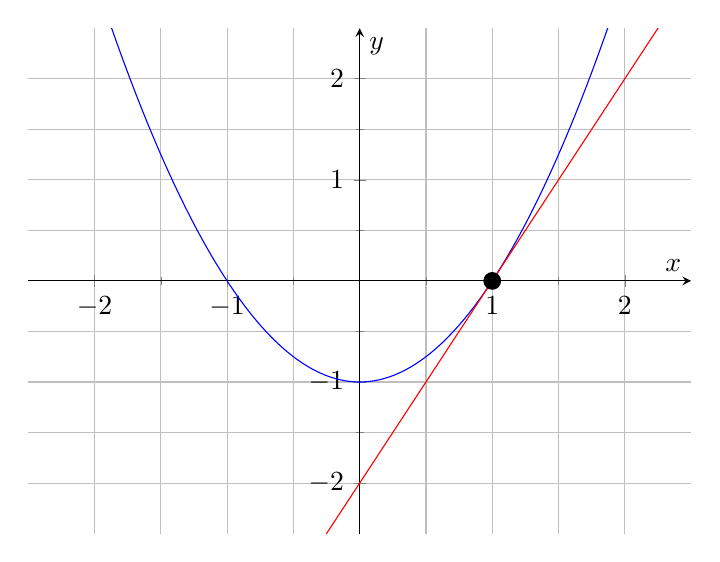
\begin{tikzpicture}
\begin{axis}[
    xlabel={$x$},
    ylabel={$y$},
    axis lines=middle,
    xmin=-2.5, xmax=2.5,
    ymin=-2.5, ymax=2.5,
    xtick={-2,-1,0,1,2},
    ytick={-2,-1,0,1,2},
    grid=both,
    minor tick num=1,
    width=10cm,
    height=8cm
]
\addplot[blue, domain=-2:2, samples=100] {x^2 - 1};
\addplot[red, domain=-1:3] {2*x - 2}; % 接線の式は点(1,1)での傾き2を使ってy = 2x - 1
\addplot[only marks, mark=*, mark options={fill=black}, mark size=3pt] coordinates {(1,0)};
\end{axis}
\end{tikzpicture}
\end{center}
 \end{exa}
   
% \begin{tcolorbox}[
%    colback = white,
%    colframe = green!35!black,
%    fonttitle = \bfseries,
%    breakable = true]
%    \begin{thm}
%$f(x)$が$x=a$で微分可能ならば$x=a$で連続である.
%\end{thm}
%  \end{tcolorbox}

 \begin{tcolorbox}[
    colback = white,
    colframe = green!35!black,
    fonttitle = \bfseries,
    breakable = true]
    \begin{prop}[微分の性質]
$f,g$を区間$I$上の微分可能な関数とするとき, 以下が成り立つ. ($c$は定数.)
 \begin{itemize}
   \setlength{\parskip}{0cm} 
  \setlength{\itemsep}{0cm}
 \item  $(f \pm g)' = f '\pm g'$.
  \item  $(c f)' = cf'$.
   \item  $(fg)' = f'g + fg'$.
    \item $ \left( \frac{f}{g} \right)' = \frac{f'g - f g'}{g^2}$.
    ($g'(x) \neq 0$なる点において.)
 \end{itemize}
 \end{prop}
   \end{tcolorbox}
 
   \begin{exa}
$f(x) = (x^2 +3)(x^{2}+1)$とすると
$f'(x) =2x(x^2 +1) + (x^2 +3)2x = 4x(x^2 +2)$.
 \end{exa}
   
   
  \begin{exa}
$f(x) = \frac{1}{x^{2}+1}$とすると
$f'(x) = - \frac{2x}{(x^2 +1)^2}$.
 \end{exa}
   
 
   
 \subsection{初等関数の微分}

   
 \begin{tcolorbox}[
    colback = white,
    colframe = green!35!black,
    fonttitle = \bfseries,
    breakable = true]
    \begin{prop}[三角関数の微分]
    \text{}
 \begin{itemize}
   \setlength{\parskip}{0cm} 
  \setlength{\itemsep}{0cm}
 \item  $(\sin x)' = \cos x$ 
 \item  $(\cos x)' = -\sin x$
  \item  $(\tan x)' = \frac{1}{(\cos x)^2}$
 \end{itemize}
 \end{prop}
   \end{tcolorbox}

    \begin{tcolorbox}[
    colback = white,
    colframe = green!35!black,
    fonttitle = \bfseries,
    breakable = true]
    \begin{prop}[指数関数・対数関数の微分]
    \text{}
 \begin{itemize}
    \setlength{\parskip}{0cm} 
  \setlength{\itemsep}{0cm}
 %\item  $\lim_{x \rightarrow 0} \frac{\log (1+x)}{x} =1$, $\lim_{x \rightarrow 0} \frac{e^x -1}{x} =1$.
 \item  $(a^x)' = (\log a) a^x$. 特に$(e^x)' = e^x$.
  \item  $(\log_{a} x)' = \frac{1}{(\log a) x}$. 特に$(\log x)' = \frac{1}{x}$.
 \end{itemize}
 \end{prop}
   \end{tcolorbox}
   
    \begin{tcolorbox}[
    colback = white,
    colframe = green!35!black,
    fonttitle = \bfseries,
    breakable = true]
    \begin{prop}[無理関数の微分]
$(x^{\alpha})' = \alpha x^{\alpha-1}$.
 \end{prop}
   \end{tcolorbox}
   
   \subsection{合成関数の微分法}
   \begin{tcolorbox}[
    colback = white,
    colframe = green!35!black,
    fonttitle = \bfseries,
    breakable = true]
    \begin{thm}[合成関数の微分法]
$y=f(x)$が$x=a$で微分可能であり, $z=g(y)$が$y=f(a)$で微分可能であるとき, 
$z=g(f(x))$は$x=a$で微分可能であり, 
$$
\drv{z}{x}=\drv{z}{y}\drv{y}{x} 
\text{\,\,である.}
$$
より詳しく書くと, 
$$\drv{z}{x}\Bigr|_{x=a}=\drv{z}{y}\Bigr|_{y=f(a)}\drv{y}{x}\Bigr|_{x=a}
\text{\,\,である.}
$$
 \end{thm}
   \end{tcolorbox}

 
  \begin{exa}
 $z=(x^2 +1)^3$の微分を合成関数の微分法で求める. 
 $y=x^2+1, z=y^3$とすると$\drv{y}{x}=2x, \drv{z}{y}=3 y^2$より, 
 $$
 \drv{z}{y}\drv{y}{x}  = 3(x^2+1)^{2} \cdot 2x=-6x(x^2+1)^{2} \text{\,\,である.}
 $$
 \end{exa}
 
 
 \begin{exa}
 $z=\cos(x^2)$の微分を合成関数の微分法で求める. 
 $y=x^2, z=\cos y$とすると$\drv{y}{x}=2x, \drv{z}{y}=-\sin (y)$より, 
 $$
 \drv{z}{y}\drv{y}{x}  = (-\sin (x^2) )2x=-2x\sin (x^2) \text{\,\,である.}
 $$
 \end{exa}
 
 \begin{exa}
 $z=x^{\alpha}=e^{\alpha \log x}$の微分を合成関数の微分法で求める. 
 $y=\alpha \log x, z=e^{y}$とすると$\drv{y}{x}=\frac{\alpha}{x}, \drv{z}{y}=e^{y}$より, 
 $$
 \drv{z}{y}\drv{y}{x}  =e^{\alpha \log x} \cdot \frac{\alpha}{x}
 =\alpha e^{\alpha \log x} \cdot e^{ - \log x}
 =\alpha e^{(\alpha -1) \log x}
 = \alpha x^{\alpha -1}
 \text{\,\,である.}
 $$
 \end{exa}

 
 \subsection{極値と平均値の定理.}
 \begin{tcolorbox}[
    colback = white,
    colframe = green!35!black,
    fonttitle = \bfseries,
    breakable = true]
    \begin{dfn}[極値]
$f(x)$を区間$I$上の関数とする.
\begin{itemize}
\item \underline{$f(x)$が$c\in I$で極大}であるとは, $c$を含む開区間$J$があって, $x \in J$かつ$x \neq c$ならば$f(x) < f(c)$となること.
このとき, \underline{$f(x)$は$c$で極大である}といい, $f(c)$の値を\underline{極大値}という.
\item \underline{$f(x)$が$c\in I$で極小}であるとは, $c$を含む開区間$J$があって, $x \in J$かつ$x \neq c$ならば$f(x) > f(c)$となること.
このとき, \underline{$f(x)$は$c$で極小である}といい, $f(c)$の値を\underline{極小値}という.
\item  極大値, 極小値の二つ合わせて\underline{極値}という.%極値をとる点$(a,b)$を\underline{極値点}という.
\end{itemize}

    \end{dfn}
\end{tcolorbox}

\begin{tcolorbox}[
    colback = white,
    colframe = green!35!black,
    fonttitle = \bfseries,
    breakable = true]
    \begin{thm}
    $f(x)$を$[a,b]$上で連続, $(a,b)$上で微分可能な関数とする.
    $f(x)$が$c \in (a,b)$で極値を持てば, $f'(c) = 0$である.
    \end{thm}
\end{tcolorbox}

\begin{tcolorbox}[
    colback = white,
    colframe = green!35!black,
    fonttitle = \bfseries,
    breakable = true]
    \begin{thm}
    $f(x), g(x)$を$[a,b]$上で連続, $(a,b)$上で微分可能な関数とする.
\begin{itemize}
\setlength{\parskip}{0cm} 
  \setlength{\itemsep}{0cm}
\item (ロルの定理) $f(a) = f(b)$ならば, $f'(c) = 0$となる$c \in (a,b)$がある.
\item (平均値の定理)
$$
f'(c) = \frac{f(b)-f(a)}{b-a}
$$
となる$c \in (a,b)$が存在する. 
%\item (コーシーの平均値の定理)
%$g(a) \neq g(b)$かつ任意の$x \in (a,b)$について$g'(x) \neq 0$ならば
%$$
%\frac{f'(c)}{g'(c)} = \frac{f(b)-f(a)}{g(b)-g(a)}
%$$
%となる$c \in (a,b)$が存在する. 
\end{itemize}

    \end{thm}
\end{tcolorbox}

\begin{tcolorbox}[
    colback = white,
    colframe = green!35!black,
    fonttitle = \bfseries,
    breakable = true]
    \begin{thm}
    $f(x)$を$[a,b]$上で連続, $(a,b)$上で微分可能な関数とする.
\begin{itemize}
\setlength{\parskip}{0cm} 
  \setlength{\itemsep}{0cm}
\item 任意の$x \in (a,b)$について$f'(x)=0$ならば$f$は$[a,b]$上で定数関数.
\item 任意の$x \in (a,b)$について$f'(x)>0$ならば$f$は$[a,b]$上で単調増加関数.
\item 任意の$x \in (a,b)$について$f'(x)<0$ならば$f$は$[a,b]$上で単調減少関数.
\end{itemize}

    \end{thm}
\end{tcolorbox}

\begin{exa}
$(\sin x)' = \cos x$より, $\sin x$は$[-\frac{\pi}{2}, \frac{\pi}{2}]$上単調増加.
\end{exa}


%\begin{tcolorbox}[
%    colback = white,
%    colframe = green!35!black,
%    fonttitle = \bfseries,
%    breakable = true]
 %   \begin{thm}[ロピタルの定理]
%    $f(x), g(x)$を点$a$の近くで定義された微分可能な関数とする.
%$\lim_{x \rightarrow a} f(x) = \lim_{x \rightarrow a} g(x) =0$かつ
%$\lim_{x \rightarrow a} \frac{f'(x)}{g'(x)}$が存在するならば, 
%$\lim_{x \rightarrow a} \frac{f(x)}{g(x)}$も存在して
%$$
%\lim_{x \rightarrow a} \frac{f(x)}{g(x)} = \lim_{x \rightarrow a} \frac{f'(x)}{g'(x)}.$$
 %   \end{thm}
%\end{tcolorbox}
%\begin{exa}$$\lim_{x \rightarrow 0} \frac{e^{2x} - \cos x}{x} \text{\,\,を求めよ.}$$
%(答.)$\lim_{x \rightarrow 0} e^{2x} - \cos x =1-1=0$かつ$\lim_{x \rightarrow 0} x=0$であり$$\lim_{x \rightarrow 0} \frac{(e^{2x} - \cos x)'}{(x)'}=\lim_{x \rightarrow 0} \frac{2 e^{2x} - \sin x}{1} =2$$であるため, ロピタルの定理から$$\lim_{x \rightarrow 0} \frac{e^{2x} - \cos x}{x} =\lim_{x \rightarrow 0} \frac{(e^{2x} - \cos x)'}{(x)'}=2$$\end{exa}



\subsection{微分を使ったグラフの書き方}

複雑な関数でも以下の手順でグラフの概形を書くことができる.


\begin{tcolorbox}[
    colback = white,
    colframe = green!35!black,
    fonttitle = \bfseries,
    breakable = true]
\begin{itemize}
\item[手順1.]  $f'(x)=0$なる$x$の値を全て求める.  具体例としてここでは$f'(-1)=f'(3)=0$とする.
\item[手順2.]  右の図(増減表)をかく.
\begin{tabular}{|c||ccccc|}
\hline
$x$ & $\cdots$ & $-1$ & $\cdots$ & $3$ & $\cdots$ \\
\hline
$f'(x)$ &  & $0$ &  & $0$ &  \\
\hline
$f(x)$  &  & $f(-1)$ &  & $f(3)$&  \\
\hline
\end{tabular}
\item[手順3.] $(-\infty, -1)$上で$f'(x)$が正か負かを調べる. これには$(-\infty, -1)$にある具体的な値(例えば$-2$など)を入れれば良い.
例えば$f'(x)$が$(-\infty, -1)$で正ならば次のように増減表に書く.
\begin{center}
\begin{tabular}{|c||ccccc|}
\hline
$x$ & $\cdots$ & $-1$ & $\cdots$ & $3$ & $\cdots$ \\
\hline
$f'(x)$ &  $\xr{+}$& $0$ &  & $0$ &  \\
\hline
$f(x)$  & $\xr{\nearrow}$  & $f(-1)$ &  & $f(3)$&  \\
\hline
\end{tabular}
\end{center}
$(-1, 3)$上でも同様に$f'(x)$が正か負かを調べる. 例えば$f'(x)$が$(-1, 3)$上で負ならば次のように増減表に書く.
\begin{center}
\begin{tabular}{|c||ccccc|}
\hline
$x$ & $\cdots$ & $-1$ & $\cdots$ & $3$ & $\cdots$ \\
\hline
$f'(x)$ &  $\xr{+}$& $0$ & $\xb{-}$ & $0$ &  \\
\hline
$f(x)$  & $\xr{\nearrow}$  & $f(-1)$ & \xb{ $\searrow$} & $f(3)$&  \\
\hline
\end{tabular}
\end{center}

\item[手順4.] 手順3を全てやることで増減表を完成させる. 例えば次のようになったとする. 
\begin{center}
\begin{tabular}{|c||ccccc|}
\hline
$x$ & $\cdots$ & $-1$ & $\cdots$ & $3$ & $\cdots$ \\
\hline
$f'(x)$ & $+$ & $0$ & $-$ & $0$ & $+$ \\
\hline
$f(x)$ & $\nearrow$ &  $f(-1)$ & $\searrow$ &$f(3)$ & $\nearrow$ \\
\hline
\end{tabular}
\end{center}

\item[手順5.] 増減表を元にグラフを作る. $\nearrow$となっている部分は右上がりに書き, $\searrow$となっている部分は右下がりにペンを走らせると良い. また$(-1, f(-1))$や$(3, f(3))$を通るところは少し平坦になるように書く. (この部分は下の例や板書を参考してください.)

\end{itemize}
\end{tcolorbox}

\begin{exa}
$y=x^3 - x$のグラフを書く. 以下$f(x) = x^3 - 3x$とおく.

[手順1.] $f'(x)=0$なる$x$を求める.
 $f'(x)=3x^2-3$より, $x =-1,1$となる. 
 
 [手順2.] 増減表をかく.
\begin{tabular}{|c||ccccc|}
\hline
$x$ & $\cdots$ & $-1$ & $\cdots$ & $1$ & $\cdots$ \\
\hline
$f'(x)$ &  & $0$ &  & $0$ &  \\
\hline
$f(x)$  &  & $2$ &  & $-2$&  \\
\hline
\end{tabular}

[手順3.] $(-\infty, -1)$上で同様に$f'(x)$が正か負かを調べる.
ここで$f'(-2)=3(-2)^2 - 3 = 9>0$より$f'(x)$は$(-\infty, -1)$上で正である. よって増減表は次のように記入する. 

\begin{center}
\begin{tabular}{|c||ccccc|}
\hline
$x$ & $\cdots$ & $-1$ & $\cdots$ & $1$ & $\cdots$ \\
\hline
$f'(x)$ & $\xr{+}$   & $0$ &  & $0$ &  \\
\hline
$f(x)$  &  $\xr{\nearrow}$  & $2$ &  & $-2$&  \\
\hline
\end{tabular}
\end{center}

[手順4.] 増減表を完成させる.

\begin{center}
\begin{tabular}{|c||ccccc|}
\hline
$x$ & $\cdots$ & $-1$ & $\cdots$ & $1$ & $\cdots$ \\
\hline
$f'(x)$ & $+$ & $0$ & $-$ & $0$ & $+$ \\
\hline
$f(x)$ & $\nearrow$ &$2$ & $\searrow$ & $-2$& $\nearrow$ \\
\hline
\end{tabular}
\end{center}


[手順5.] 増減表を元にグラフを完成させる. 
コツとしては極値$(-1,2)$や$(1,-2)$のところに黒点を次のように書いておくと良い.  

\begin{center}
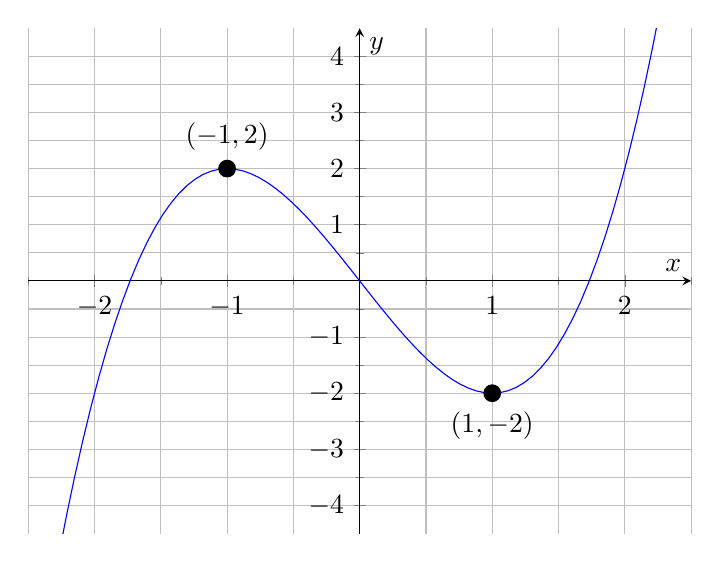
\begin{tikzpicture}
\begin{axis}[
    xlabel={$x$},
    ylabel={$y$},
    axis lines=middle,
    xmin=-2.5, xmax=2.5,
    ymin=-4.5, ymax=4.5,
    xtick={-3,-2,-1,0,1,2,3},
    ytick={-4,-3,-2,-1,0,1,2,3,4},
    grid=both,
    minor tick num=1,
    width=10cm,
    height=8cm
]
\addplot[blue, domain=-3:3, samples=100] {x^3 - 3*x};
\addplot[only marks, mark=*, mark options={fill=black}, mark size=3pt] coordinates {(-1,2)};
\node[label={90:{$(-1,2)$}},circle,fill,inner sep=2pt] at (axis cs:-1,2) {};
\addplot[only marks, mark=*, mark options={fill=black}, mark size=3pt] coordinates {(1,-2)};
\node[label={-90:{$(1,-2)$}},circle,fill,inner sep=2pt] at (axis cs:1,-2) {};
\end{axis}
\end{tikzpicture}
\end{center}

特にグラフを書くことで, $[-\frac{3}{2}, \frac{3}{2}]$上での最大値は2で最小値は-2であることがわかる. 
\end{exa}
   
   
\section{1変数の微分 -2階以上の微分-}
\subsection{高次導関数}

\begin{tcolorbox}[
    colback = white,
    colframe = green!35!black,
    fonttitle = \bfseries,
    breakable = true]
    \begin{dfn}[高次導関数の定義]
$f(x)$を区間$I$上の微分可能な関数とする.
$f'(x)$が$I$上で微分可能であるとき, \underline{$f$は2回微分可能}であるといい, 
$$
f''(x) = (f'(x)  )'
$$
としてこれを\underline{2次の導関数}と呼ぶ.
$f''(x)$は$f^{(2)}(x)$とも書く.

\hspace{12pt}同様に$f^{(n-1)}(x)$が微分可能であるとき, \underline{$f$は$n$回微分可能}であるといい, 
\underline{$n$次導関数} $f^{(n)}(x)$を$(f^{(n-1)}(x))'$として定める.
 $f^{(n)}(x)$は$\drv{^n f}{x^n}$とも書く.
    \end{dfn}
\end{tcolorbox}

\begin{exa}
\begin{itemize}
\item $f(x) = e^x$とすると, $  f^{(n)}(x) = e^x$である.
\item $f(x) = \sin x$とすると, 
   $$
  f^{(n)}(x)= \begin{cases}
(-1)^m \sin x& (n = 2m) \\
   (-1)^m \cos x& (n = 2m+1)
  \end{cases}
  \text{\,\,である.}
  $$
\end{itemize}
\end{exa}

\begin{tcolorbox}[
    colback = white,
    colframe = green!35!black,
    fonttitle = \bfseries,
    breakable = true]
    \begin{dfn}[$C^n$級関数]
$f(x)$を区間$I$上の関数とする.
\begin{itemize}
  \setlength{\parskip}{0cm} 
  \setlength{\itemsep}{0cm}
\item $f(x)$が$n$回微分可能であり, $f^{(n)}(x)$が連続であるとき, 
\underline{$f$は$C^n$級関数}であるという.
\item 任意の$n \in \N$について$f$が$C^n$級であるとき, 
\underline{$f$を$C^{\infty}$級関数}であるという.
\end{itemize}

    \end{dfn}
\end{tcolorbox}

\begin{exa}
みんながよく知っている関数は(だいたい)$C^{\infty}$級関数. 
つまり$x^2,\sin x, \cos x, e^x $などは$C^{\infty}$級関数である.
\end{exa}


\subsection{テイラーの定理とその応用}

\begin{tcolorbox}[
    colback = white,
    colframe = green!35!black,
    fonttitle = \bfseries,
    breakable = true]
    \begin{thm}[テイラーの定理 1]
$f(x)$が開区間$I$上の$C^2$級関数とする.
$a<b$なる$a,b \in I$について
$$
f(b) = f(a) + f'(a) (b-a) + \frac{f''(c)}{2}(b-a)^2
$$
となる$c \in (a,b)$が存在する.
    \end{thm}
\end{tcolorbox}

\begin{exa}
$f(x) = e^x$とし$a=0$かつ$b$を正の実数とする.
このときある$c \in (0,b)$があって
$$
e^b = f(0) + f'(0) b + \frac{f''(c)}{2}b^2
= 1 + b + \frac{e^c}{2} b^2
$$
となる. $e^c \geqq 1$であるため, 
$$
e^b \geqq  1 + b + \frac{1}{2} b^2 \text{\,\,となる.}
$$
\end{exa}

\begin{tcolorbox}[
    colback = white,
    colframe = green!35!black,
    fonttitle = \bfseries,
    breakable = true]
    \begin{thm}[極値判定法]
$f(x)$が点$a$の周りで定義された$C^2$級関数とする.
\begin{itemize}
  \setlength{\parskip}{0cm} 
  \setlength{\itemsep}{0cm}
\item $f'(a) = 0$かつ$f''(a)>0$なら$f(x)$は$x=a$で極小.
\item $f'(a) = 0$かつ$f''(a) < 0$なら$f(x)$は$x=a$で極大.
\end{itemize}
    \end{thm}
\end{tcolorbox}

\begin{tcolorbox}[
    colback = white,
    colframe = green!35!black,
    fonttitle = \bfseries,
    breakable = true]
    \begin{thm}[テイラーの定理 2]
$f(x)$が開区間$I$上の$C^n$級関数とする.
$a<b$なる$a,b \in I$について
$$
f(b) = f(a) + f'(a) (b-a) + \frac{f''(a)}{2!}(b-a)^2 + \cdots 
+  \frac{f^{(n-1)}(a)}{(n-1)!}(b-a)^{n-1} + \frac{f^{(n)}(c)}{n!}(b-a)^{n}
$$
となる$c \in (a,b)$が存在する.
    \end{thm}
\end{tcolorbox}

\begin{exa}
$f(x) = e^x$とし$a=0$かつ$b$を正の実数とする.
このときある$c \in (0,b)$があって
\begin{align*}
\begin{split}
e^b &= f(0) + f'(0) b + \frac{f''(0)}{2!}b^2 +  \cdots +\frac{f^{(n-1)}(0)}{(n-1)!}b^{n-1} + \frac{f^{(n)}(c)}{n!}b^{n} \\
&= 1 + b + \frac{1}{2!} b^2 + \frac{1}{3!} b^3 + \cdots 
+ \frac{1}{(n-1)!}b^{n-1}  + \frac{e^c}{n!}b^{n} 
\end{split}
\end{align*}
となる. $e^c \geqq 1$であるため, 
$$
e^b \geqq  1 + b + \frac{1}{2!} b^2 + \frac{1}{3!} b^3 + \cdots 
+ \frac{1}{(n-1)!}b^{n-1}  + \frac{1}{n!}b^{n} 
\text{\,\,となる.}
$$
\end{exa}

\begin{tcolorbox}[
    colback = white,
    colframe = green!35!black,
    fonttitle = \bfseries,
    breakable = true]
    \begin{thm}[有限テイラー展開]
$f(x)$が開区間$I$上の$C^n$級関数とする.
$a \in I$を固定する.
任意の$x \in I$について, ある$\theta \in (0,1)$があって
\begin{align*}
\begin{split}
f(x) &= f(a) + f'(a) (x-a) + \frac{f''(a)}{2!}(x-a)^2 + \cdots \\
&\cdots +  \frac{f^{(n-1)}(a)}{(n-1)!}(x-a)^{n-1} + \frac{f^{(n)}(a + \theta(x-a))}{n!}(x-a)^{n} \\
&=\sum_{k=0}^{n-1}\frac{f^{(k)}(a)}{k!}(x-a)^k + \frac{f^{(n)}(a + \theta(x-a))}{n!}(x-a)^{n}
\end{split}
\end{align*}
となる.
右辺を$x=a$における\underline{有限テーラー展開}と呼び, 
$R_n=\frac{f^{(n)}(a + \theta(x-a))}{n!}(x-a)^{n}$を\underline{剰余項}と呼ぶ.
特に$a=0$のとき, \underline{有限マクローリン展開}と呼ぶ.
    \end{thm}
 \end{tcolorbox}
    
\begin{exa}
任意の$x \in \R$についてある$\theta \in (0,1)$があって
$$
\sin x = 1 - \frac{x^3}{3!} + \frac{x^5}{5!} - \cdots  + 
 \frac{(-1)^{n-1} x^{2n-1}}{(2n-1)!} 
 + \frac{ (-1)^n x^{2n}\sin (\theta x) }{2n!}
$$
となる.

\end{exa}

\begin{tcolorbox}[
    colback = white,
    colframe = green!35!black,
    fonttitle = \bfseries,
    breakable = true]
    \begin{thm}[べき級数展開]
$f(x)$を$a$を含む開区間上の$C^{\infty}$級関数とする.
テイラーの定理
$$
f(x)=\sum_{k=0}^{n-1}\frac{f^{(k)}(a)}{k!}(x-a)^k + \frac{f^{(n)}(a + \theta(x-a))}{n!}(x-a)^{n}
$$
において, 剰余項$R_n(x)=\frac{f^{(n)}(a + \theta(x-a))}{n!}(x-a)^{n}$とする.
ある区間$I$とし$x\in I$において$\lim_{n \rightarrow \infty}|R_n(x)| =0$となるならば,
$$
f(x)=\sum_{k=0}^{ \infty }\frac{f^{(k)}(a)}{k!}(x-a)^k  \text{\,\,\, となる.}
$$
    \end{thm}
 \end{tcolorbox}
 \begin{exa}
 $f(x)=e^x$とし, $a=0$とする. このとき剰余項は
 $$
 R_n(x) = \frac{e^{ \theta x} x^n}{n!}
 $$
 である. 例\ref{exa-frac}より$\lim_{n \rightarrow \infty}|R_n(x)| =0$であるので, べき級数展開ができ, 
\begin{align*}
\begin{split}
e^x &= \sum_{k=0}^{ \infty }\frac{f^{(k)}(a)}{k!}x^k = 1 + x + \frac{x^2}{2!} + \frac{x^3}{3!} + \frac{x^4}{4!} + \cdots 
\end{split}
\end{align*}
 \end{exa}
 
  \begin{exa}
 $f(x)=\sin x$とし, $a=0$とする. このとき剰余項は
 $$
 R_{2n}(x) = \frac{(-1)^{n}x^{2n} \sin ( \theta x) }{(2n)!}
 $$
 である. $\lim_{n \rightarrow \infty}|R_n(x)| =0$であるので, べき級数展開ができ, 
\begin{align*}
\begin{split}
\sin x&= \sum_{k=0}^{ \infty }\frac{f^{(k)}(a)}{k!}x^k = 
 x - \frac{x^3}{3!} + \frac{x^5}{5!} -  \frac{x^7}{7!} +  \cdots 
\end{split}
\end{align*}
 \end{exa}
 
 \subsection{初等関数の冪級数展開}

 初等関数の$x=0$における冪級数展開は次のとおりとなる. 
\begin{align*}
\begin{split}
e^x &= 1 + x+  \frac{x^2}{2!} + \frac{x^3}{3!}  + \cdots  + 
 \frac{ x^{n}}{n!} + \cdots \\
\sin x &= x - \frac{x^3}{3!} + \frac{x^5}{5!} - \cdots  + 
 \frac{(-1)^{n-1} x^{2n-1}}{(2n-1)!} 
 +\cdots \\
 \cos x &= 1 - \frac{x^2}{2!} + \frac{x^4}{4!} - \cdots  + 
 \frac{(-1)^{n} x^{2n}}{(2n)!} 
 + \cdots\\
 \log(1+x) &= x - \frac{x^2}{2} + \frac{x^3}{3}  - \cdots   
 + \frac{ (-1)^{n-1}x^{n}}{n!} + \cdots \\
 % \sinh x &= x + \frac{x^3}{3!} + \frac{x^5}{5!} + \cdots  + \frac{x^{2n-1}}{(2n-1)!} + o(x^{2n-1}) \text{\,\,\,}(x \rightarrow 0) \\
\end{split}
\end{align*}
初等関数であっても綺麗に漸近展開できるとは限らない. 例えば$\tan x$などの漸近展開の一般項は非常に難しい.
 
次の定理はこの授業の範囲外の内容だが, 面白いので書いておく. 
\begin{tcolorbox}[
    colback = white,
    colframe = green!35!black,
    fonttitle = \bfseries,
    breakable = true]
    \begin{thm}[オイラーの公式]
$i$を虚数($i^2=1$となる数)とするとき, 
$$
e^{ix} = \cos x + i \sin x.
$$
特に次が成り立つ.
$$
e^{i \pi} =-1
$$
    \end{thm}
 \end{tcolorbox}
 
\section{1変数の積分}


    
      \begin{tcolorbox}[
    colback = white,
    colframe = green!35!black,
    fonttitle = \bfseries,
    breakable = true]
    \begin{dfn}
関数$F(x)$が微分可能であり$\drv{F}{x} = f(x)$となるとき, 
$F(x)$を\underline{$f(x)$の不定積分}あるいは\underline{原始関数}といい
$$F(x) = \int f(x) dx$$
とあらわす.  

$f(x)$の不定積分は定数を除いてただ一つに定まるため, 2つの不定積分の差となる定数を\underline{積分定数}という
        \end{dfn}
    \end{tcolorbox}

\begin{exa}
$n$を$-1$でない整数とする. 
このとき$x^n$の不定積分は
$\int x^n dx = \frac{x^{n+1}}{n+1} +C$となる. ただし$C$は積分定数とする. 
\end{exa}

 \begin{exa}
簡単な不定積分に関してまとめておく.
積分定数に関しては省略する.
  \begin{align*}
\begin{split}
\int x^\alpha \,dx &= \frac{x^{\alpha+1}}{\alpha+1} \text{\,\,\, ($\alpha \neq -1$のとき)}\\
\int \frac{1}{x} \,dx &= \log |x|\\
%\int \frac{1}{\sqrt{a^2 - x^2}} \,dx &= \Sin \frac{x}{|a|} \text{\,\,\, ($a \neq 0$のとき)}\\
%\int \frac{1}{a^2 + x^2} \,dx &= \frac{1}{a}\Tan \frac{x}{a} \text{\,\,\, ($a \neq 0$のとき)}\\
\int e^x \,dx &=e^x\\
\int a^x \,dx &=\frac{1}{\log a}a^x \text{\,\,\, ($a>0$かつ$a \neq 1$のとき)} \\
\int \log x  \,dx &=x \log x -x\\
\int \sin x  \,dx &=-\cos x \\
\int \cos x  \,dx &=\sin x \\
\int \frac{1}{(\cos x)^2}  \,dx &=\tan x \\
\end{split}
\end{align*}
 \end{exa}
 
      \begin{tcolorbox}[
    colback = white,
    colframe = green!35!black,
    fonttitle = \bfseries,
    breakable = true]
    \begin{dfn}[積分の感覚的な定義]
$f(x)$を$[a,b]$上の連続関数とする.
曲線$y=f(x)$と直線$x=a, x=b$それに$x$軸で囲まれた部分の面積を, 
$x$軸より上の部分は正, $x$軸より下の部分は負として加えたものを
$$
\int_{a}^{b} f(x) dx
$$
とかき\underline{$f(x)$の区間$[a,b]$における定積分}, あるいは$f(x)$を$x$で$a$から$b$まで積分するという. 


また$a < b$のとき
$$
\int_{b}^{a} f(x) dx = - \int_{a}^{b} f(x) dx
$$
と定義する. 
  \end{dfn}
  \end{tcolorbox} 
「$x$軸より上の部分は正, $x$軸より下の部分は負として加えたもの」のイメージとしては下図のような感じである. 
    \begin{figure}[htbp]
\begin{center}
 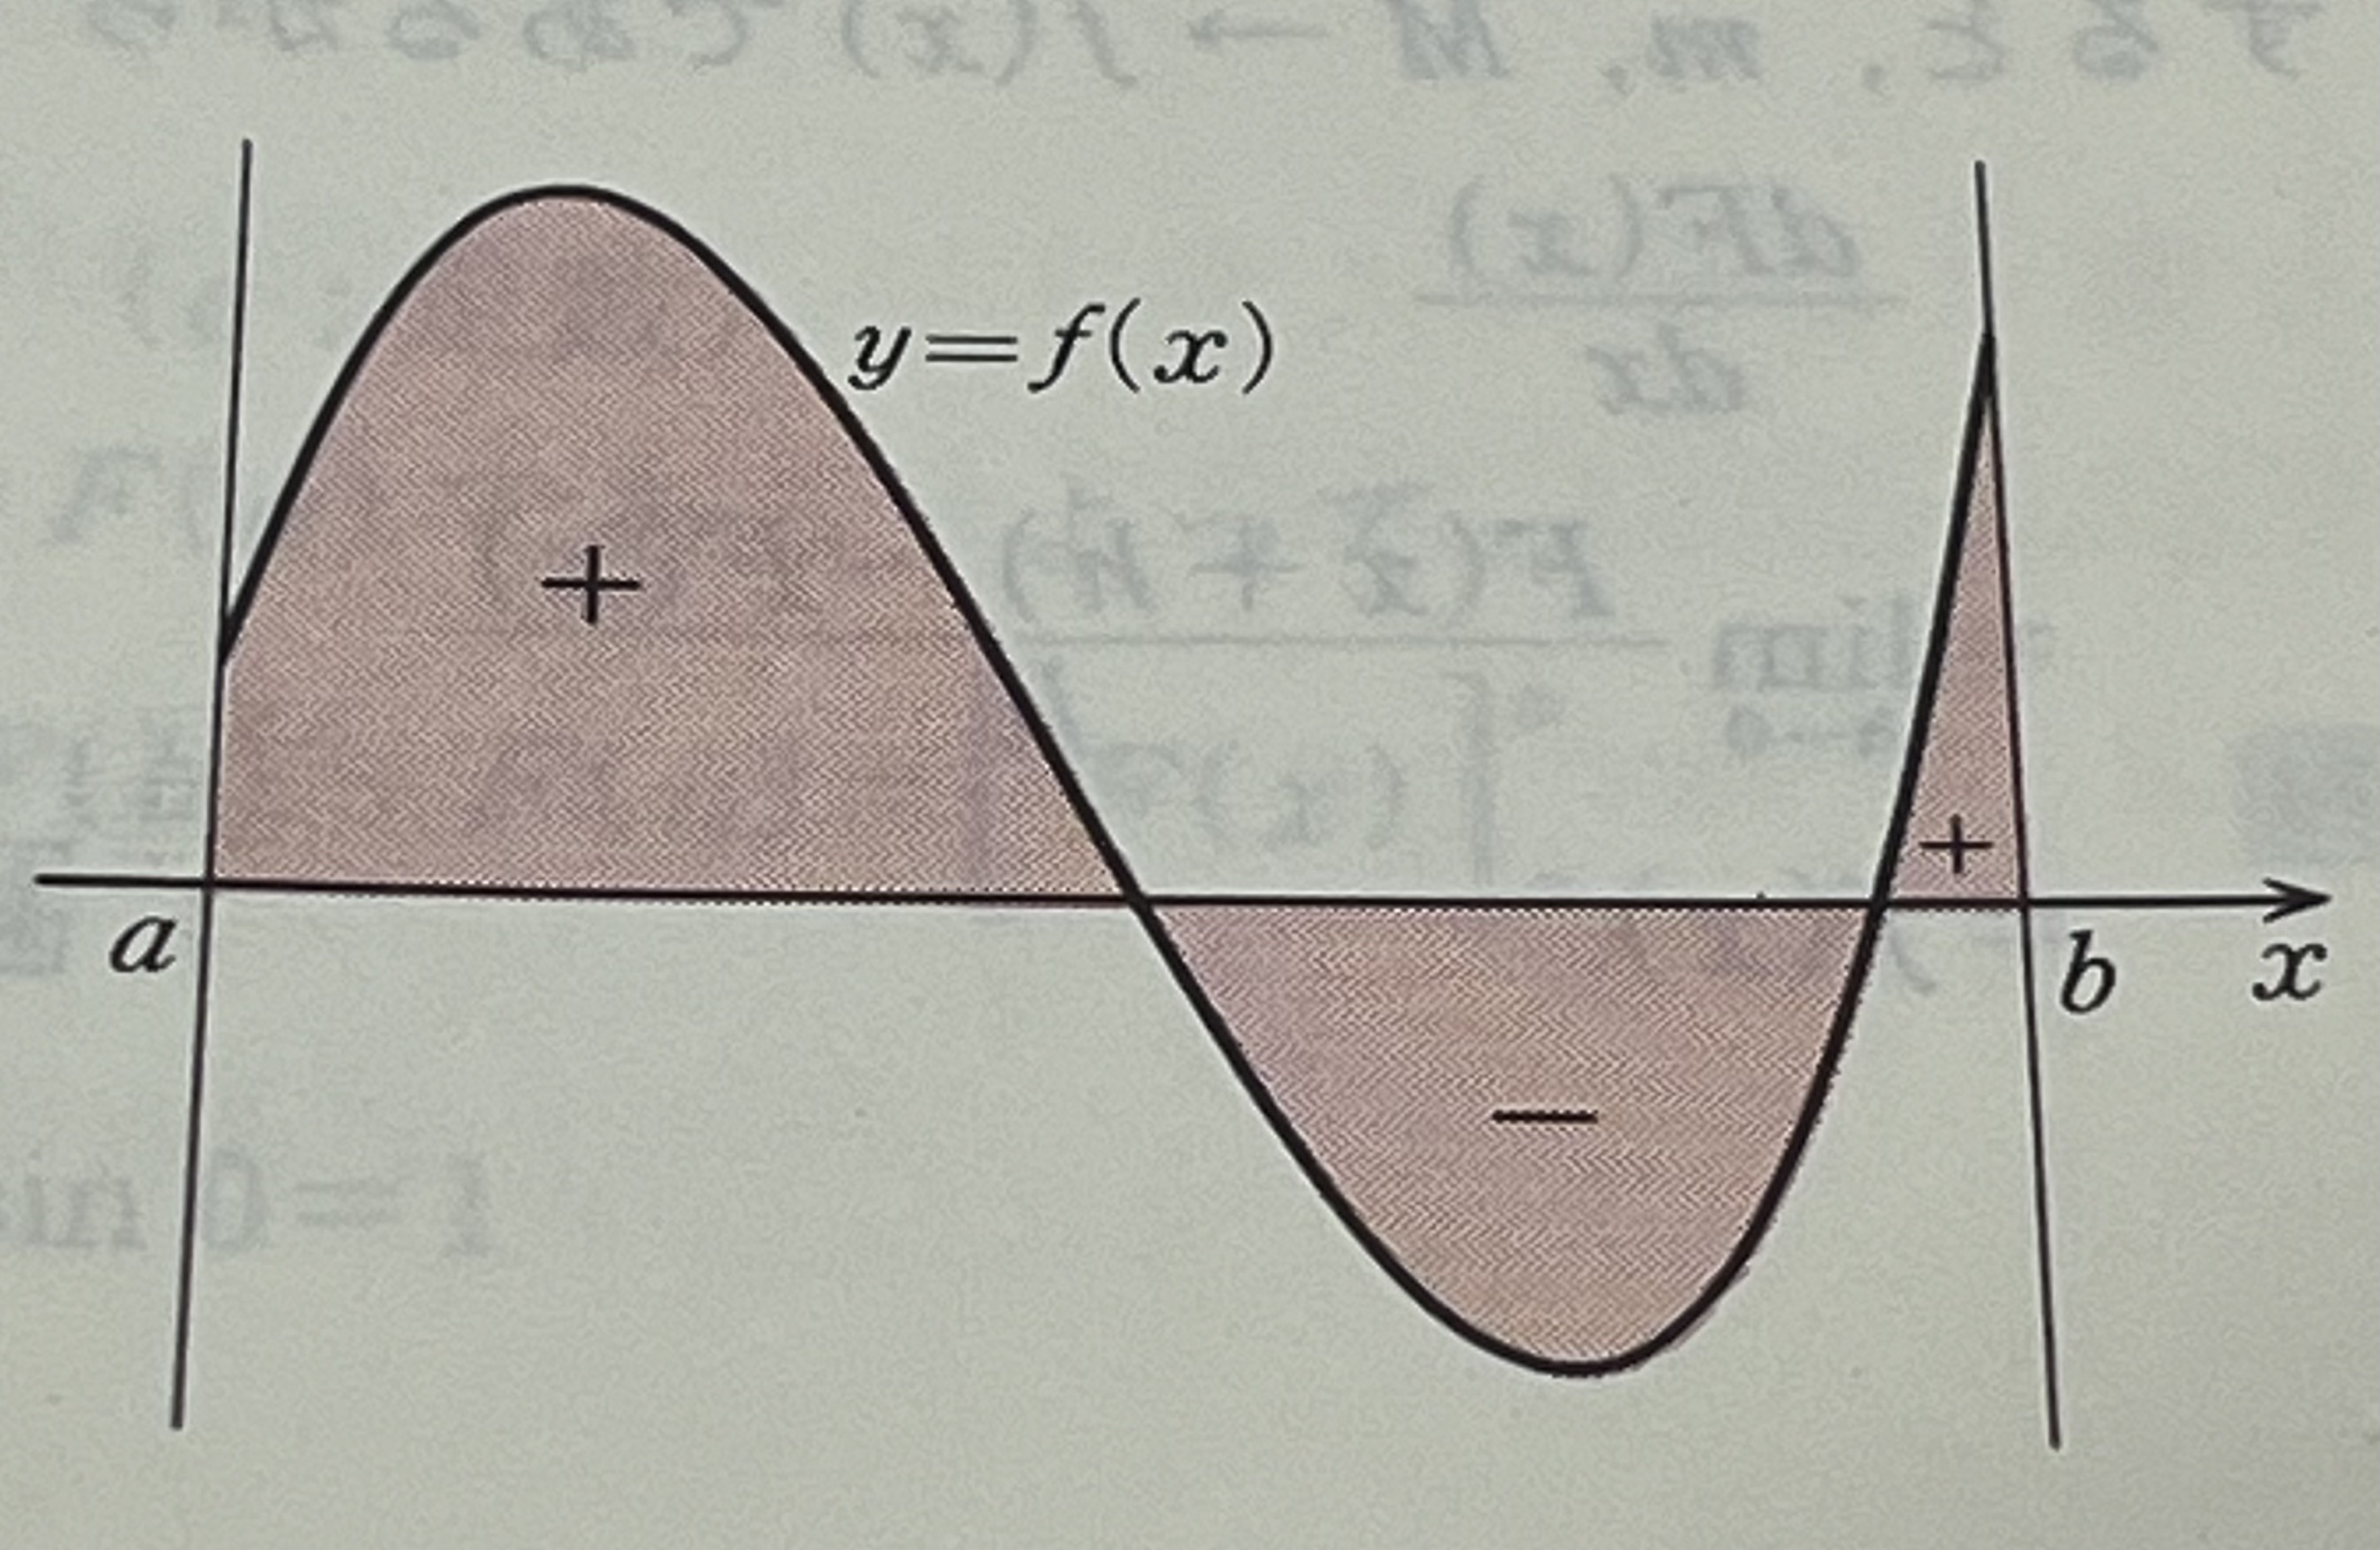
\includegraphics[height=40mm, width=60mm]{int.jpg}
\end{center}
\end{figure}
    
      \begin{tcolorbox}[
    colback = white,
    colframe = green!35!black,
    fonttitle = \bfseries,
    breakable = true]
    \begin{thm}[微分積分学の基本定理]
    $f(x)$を区間$I$上の連続関数とする.
$F(x) = \int_{a}^{x} f(x) dx$とおくと$F(x)$は$f(x)$の不定積分である. 
つまり
$$
\drv{}{x}F(x) = f(x) \text{\,\,\,である.}
$$

特に
$$
\int_{a}^{b} f(x) dx = \Bigl[ F(x) \Bigr]_{a}^{b} = F(b) - F(a) \text{\,\,\,となる.}
$$
        \end{thm}
    \end{tcolorbox}
  特に積分して微分したら元に戻る.
   つまり接線を求める微分と面積を求める積分は互いに逆の演算をしていることがわかる. 


\begin{exa}
$$\int^{1}_{0} x^2 dx = \left[\frac{x^3}{3}\right]^{1}_{0} =\frac{1}{3}.$$
図形的な意味としては$y=x^2$と直線$x=0, x=1$それに$x$軸で囲まれた部分の面積が上の量であるということである.  
\end{exa}


\begin{exa}
\label{exa-area-2}
$M$を1以上の定数とすると, 
$$\int^{M}_{1} \frac{1}{x^2} dx = \left[-\frac{1}{x}\right]^{M}_{1} =1 - \frac{1}{M}.$$
 図形的な意味としては$y=\frac{1}{x^2}$と直線$x=1, x=M$それに$x$軸で囲まれた部分の面積が上の量であるということである. 
 \end{exa}

\begin{exa}
\label{exa-area-1}
$M$を1以上の定数とすると, 
$$\int^{M}_{1} \frac{1}{x} dx = \left[\log |x|\right]^{M}_{1} = \log M.$$
 図形的な意味としては$y=\frac{1}{x}$と直線$x=1, x=M$それに$x$軸で囲まれた部分の面積が上の量であるということである.  
\end{exa}

\begin{exa}
$1 + \frac{1}{2}+ \frac{1}{3}+ \frac{1}{4}+ \frac{1}{5}+\cdots$は$+ \infty$に発散するが, 
 $1 + \frac{1}{4}+ \frac{1}{9}+ \frac{1}{16}+ \frac{1}{25}+ \cdots$は収束する. 
ちなみに
$$
\frac{\pi^2}{6} =  1 + \frac{1}{4}+ \frac{1}{9}+ \frac{1}{16}+ \frac{1}{25}+\cdots
$$
 であることが知られている. 
\end{exa}


    \begin{tcolorbox}[
    colback = white,
    colframe = green!35!black,
    fonttitle = \bfseries,
    breakable = true]
    \begin{prop}[積分の性質]
$f(x), g(x)$共に$[a,b]$上の連続関数とし, $G(x) = \int g(x) dx$とする.
\begin{enumerate}
\item $\int_{a}^{b} (f(x) \pm g(x)) dx = \int_{a}^{b} f(x) dx \pm \int_{a}^{b} g(x) dx$
\item $k$を定数とするとき, $\int_{a}^{b} kf(x) dx  = k \int_{a}^{b} f(x) dx $
\item (置換積分法)    $$
\begin{array}{cccc}
x(t): &[\alpha, \beta]& \rightarrow & [a,b]\\
&t& \longmapsto & x(t)
\end{array}
$$
を$C^{\infty}$級関数とし, $a = x(\alpha), b=x(\beta)$とするとき
$$
\int_{a}^{b} f(x) dx = \int_{\alpha}^{\beta} f(x(t)) \drv{x(t)}{t} dt \text{\,\,\,となる.}
$$
\item (部分積分法)  $f(x)$が$C^{\infty}$級であるとき,
$$
\int_{a}^{b} f(x) g(x)dx = \Bigl[ f(x) G(x)\Bigr]^{b}_{a} - \int_{a}^{b}f'(x) G(x)dx
\text{\,\,\,となる.}$$
\end{enumerate}
        \end{prop}
    \end{tcolorbox}
 
  \begin{exa}
 \label{exa-area-1}
 $ \int (\sin x)^2 \cos x dx $は$t = \sin x$という置換積分を用いると次のように求められる.(積分定数は省略する).
 $$
 \int (\sin x)^2 \cos x dx 
 = \int t^2 \drv{t}{x} dx
  = \int t^2 dt
  = \frac{t^3}{3}
  =\frac{(\sin x)^3}{3}
 $$
\end{exa}
 
 \begin{exa}
 $\int \log x dx$は部分積分法を用いて次のように求められる. (積分定数は省略する).
 $$
 \int \log x dx 
 = \int x' \log x dx
 = x \log x - \int x (\log x)' dx
 = x \log x - \int 1 dx
 = x \log x - x
 $$
\end{exa}
  

\section{2変数の微分}


\subsection{偏微分}



以下この授業・資料においては, 領域$D$といえば
$$D=(a,b) \times (c,d) =\{ (x,y) \in \R^2 | a < x <b, c<y<d\}$$
を指すことにする. 

 \begin{tcolorbox}[
    colback = white,
    colframe = green!35!black,
    fonttitle = \bfseries,
    breakable = true]
    \begin{dfn}[]
$D$を$\R^2$の領域とする.
 任意の$(x,y) \in D$について, 実数$f(x)$がただ一つ定まるとき, 
 \underline{$f(x)$を$D$上の関数}といい
    $$
\begin{array}{cccc}
f: &D& \rightarrow & \R  \\
&(x,y)& \longmapsto & f(x,y)
\end{array}
\text{\,\,と書く.}
$$
\end{dfn}
\end{tcolorbox}



\begin{rem}
この授業において$f(x,y)$の連続性や全微分可能性など難しいことはやらないことにする.
授業の内容を簡単にするため以後は以下を仮定する.
\begin{tcolorbox}[
    colback = white,
    colframe = green!35!black,
    fonttitle = \bfseries,
    breakable = true]
[仮定.] 任意の$(a,b) \in D$について,
$f(x,b)$は$x$の関数と見て$C^{\infty}$級, つまり何回でも微分可能であるものとする.
同様に$f(a,y)$は $y$の関数と見て$C^{\infty}$級であるものとする.
このような関数$f$は\underline{$C^{\infty}$級関数}と呼ばれる.
\end{tcolorbox}

\end{rem}


\begin{tcolorbox}[
    colback = white,
    colframe = green!35!black,
    fonttitle = \bfseries,
    breakable = true]
    \begin{dfn}
    \label{partial}
    任意の$(a,b) \in D$について,
    $$A = \lim_{x \rightarrow a} \frac{f(x,b) - f(a,b)}{x-a} \text{,\,\, \,\,} 
    B = \lim_{y \rightarrow b}\frac{f(a,y) - f(a,b)}{y-b} $$
   とする.  $A,B$を\underline{$f(x,y)$の$(a,b)$での偏微分係数}と呼び, 
    $$A=\pdrv{f}{x}(a,b)    \text{,\,\, \,\,} B=\pdrv{f}{y}(a,b)\text{\,\,とかく.\,\,}$$

    \end{dfn}
\end{tcolorbox}
$\pdrv{f}{x}(a,b) $は$\pdrv{f}{x}|_{(x,y)=(a,b)}$とかくこともある.




\begin{tcolorbox}[
    colback = white,
    colframe = green!35!black,
    fonttitle = \bfseries,
    breakable = true]
    \begin{dfn}
    $D$上で$C^{\infty}$級関数$f$について
    
   $$
\begin{array}{ccccccccc}
\pdrv{f}{x}: &D & \rightarrow & \R & &\pdrv{f}{y}: &D & \rightarrow & \R \\
&(x,y) & \longmapsto & \pdrv{f}{x}(x,y)& & &(x,y) & \longmapsto & \pdrv{f}{y}(x,y)
\end{array}
$$
    
を\underline{$f(x,y)$の偏導関数}という.
     
    \end{dfn}
    
\end{tcolorbox}


\begin{exa}
\begin{itemize}

\item $f(x,y) = x^2y^3$は$\R^2$の偏導関数は
$\pdrv{f}{x} = 2xy^3, \pdrv{f}{y} = 3x^2y^2 $である.
\item $f(x,y) = \sqrt{1-x^2-y^2}$は$\{ (x,y) \in \R^2 : \sqrt{x^2 + y^2} <1 \}$の偏導関数は
$$\pdrv{f}{x} = \frac{-x}{\sqrt{1-x^2-y^2}}\text{,\,\,\,\,}
\pdrv{f}{y} = \frac{-y}{\sqrt{1-x^2-y^2}}\text{\,\,である.\,\,}$$
\end{itemize}
\end{exa}

\begin{tcolorbox}[
    colback = white,
    colframe = green!35!black,
    fonttitle = \bfseries,
    breakable = true]
    \begin{thm}[接平面の方程式]
   $f (x,y)$を領域$D$上の$C^{\infty}$関数とする.
   曲面$z =f(x,y)$の点$(a,b)$での接平面の方程式は次で与えられる.
   $$
  z - f(a,b) = \pdrv{f}{x}(a,b) (x-a) + \pdrv{f}{y}(a,b)(y-b) 
   $$
     
    \end{thm}
    
\end{tcolorbox}

\begin{exa}
$f(x,y) = -(x^2+ y^2)$の点$(0,0)$での偏微分係数は
$A=\pdrv{f}{x}(0,0) =0$, $B=\pdrv{f}{y}(0,0) =0$.
接平面の方程式は
$z=0+A(x-0)+B(y-0)=0$.

 
\end{exa}

\subsection{連鎖律}

\begin{tcolorbox}[
    colback = white,
    colframe = green!35!black,
    fonttitle = \bfseries,
    breakable = true]
    \begin{thm}
    
    $f(x,y)$を領域$D$上の$C^{\infty}$級関数とする.
    $x=x(t)$, $y=y(t)$を$t$に関する$C^{\infty}$級関数とし, $z(t) = f(x(t) , y(t))$とするとき, 
    $$
    \drv{z}{t} = \pdrv{f}{x}\drv{x}{t} + \pdrv{f}{y}\drv{y}{t}.
    $$
    \end{thm}
    \end{tcolorbox}

\begin{exa}
$f(x,y) = 2x^3y$, $x(t) = \cos t$, $y(t) = \sin t$, 
 $z(t) = f(x(t) , y(t))$とする.
 このとき
 $$
 \pdrv{f}{x} = 6x^2y,  \pdrv{f}{y}=2x^3, \drv{x}{t}=-\sin t, \drv{y}{t}=\cos t\text{,\,\, より}
 $$
 \begin{align*}
 \begin{split}
     \drv{z}{t} & = \pdrv{f}{x}\drv{x}{t} + \pdrv{f}{y}\drv{y}{t}
     = 6\cos^2 t\sin t (-\sin t) + 2 \cos^3 t \cos t
     = - 6\cos^2 t\sin^2 t  + 2 \cos^4 t.
   \end{split}
 \end{align*}
 
\end{exa}


\begin{tcolorbox}[
    colback = white,
    colframe = green!35!black,
    fonttitle = \bfseries,
    breakable = true]
    \begin{dfn}
    
    領域$D$上の$C^{\infty}$級関数を$x(u,v)$, $y(u,v)$とする.
    
 $$
\begin{array}{ccccc}
\Phi: &D & \rightarrow & \R^2 & \\
&(u,v) & \longmapsto & (x(u,v),y(u,v))&
\end{array}
$$
を$C^{\infty}$級変数変換という.
    \end{dfn}
    \end{tcolorbox}


\begin{exa}
\begin{itemize}
\item $a,b,c,d$を定数とする.
$\Phi(u,v)  = (au+bv, cu+dv)$は$C^{\infty}$級変数変換である.
これを1次変換という.
\item $\Phi(u,v)  = (u \cos v, u \sin v)$も$C^{\infty}$級変数変換である.
これを極座標変換という.
\end{itemize}

\end{exa}


\begin{tcolorbox}[
    colback = white,
    colframe = green!35!black,
    fonttitle = \bfseries,
    breakable = true]
    \begin{thm}
 領域$D$上の$C^{\infty}$級変数変換を
 $$
\begin{array}{ccccc}
\Phi: &D & \rightarrow & \R^2 & \\
&(u,v) & \longmapsto & (x(u,v),y(u,v))&
\end{array}
$$
とし, 領域$E ( \subset \Phi(D))$上の$C^{\infty}$級関数を$f(x,y)$とする.

 領域$D$上の$C^{\infty}$級$g(u,v)$を
 $$
\begin{array}{ccccc}
g = f \circ \Phi: &D & \rightarrow & \R & \\
&(u,v) & \longmapsto & f(x(u,v),y(u,v))&
\end{array}
$$
で定めるとき, 各偏導関数は以下の通りになる.

    $$
    \pdrv{g}{u} = \pdrv{f}{x}\pdrv{x}{u} + \pdrv{f}{y}\pdrv{y}{u}
    \text{,\,\,\, \,\,\,\,\,\,\,}
     \pdrv{g}{v} = \pdrv{f}{x}\pdrv{x}{v} + \pdrv{f}{y}\pdrv{y}{v}.
    $$
    \end{thm}
    \end{tcolorbox}
行列の記法を用いると以下のようにかける. (行列に関しては後期の授業を参考にすること.)
$$
\left( \pdrv{g}{u}  , \pdrv{g}{v}\right) 
=
\left( \pdrv{f}{x} , \pdrv{f}{y}\right) 
\left(\begin{array}{cc} \pdrv{x}{u} & \pdrv{x}{v} \\ \pdrv{y}{u}& \pdrv{y}{v} \\ \end{array} \right).
$$
\begin{exa}
$f(x,y)$を$C^{\infty}$級関数とし,$C^{\infty}$級変数変換を$(x(u,v),y(u,v)) = (u \cos v, u \sin v)$とする.
$g(u,v) = f(x(u,v), y(u,v))$とするとき, $\pdrv{g}{u}, \pdrv{g}{v}$を
$\pdrv{f}{x},\pdrv{f}{y}$を用いてあらわせ.

(解.)
$$
\pdrv{x}{u}=\cos v,\text{\,\,} \pdrv{x}{v}= -u\sin v,\text{\,\,}  \pdrv{y}{u}=\sin v,\text{\,\,}  \pdrv{y}{v}= u \cos v, \text{\,\,\,より} 
$$
$$
   \pdrv{g}{u} = \pdrv{f}{x}\pdrv{x}{u} + \pdrv{f}{y}\pdrv{y}{u}=\cos v\pdrv{f}{x} + \sin v\pdrv{f}{y}.
$$

$$
  \pdrv{g}{v} = \pdrv{f}{x}\pdrv{x}{v} + \pdrv{f}{y}\pdrv{y}{v}
   =-u\sin v \pdrv{f}{x} + u \cos v\pdrv{f}{y}.
$$
\end{exa}
\subsection{2階偏導関数}

\begin{tcolorbox}[
    colback = white,
    colframe = green!35!black,
    fonttitle = \bfseries,
    breakable = true]
    \begin{dfn}
$f(x,y)$を$C^{\infty}$級関数とする.
\begin{itemize}
\item $\pdrv{f}{x} , \pdrv{f}{y}$を\underline{$f$の1階偏導関数}という.
\item $\pdrv{f}{x} , \pdrv{f}{y}$の導関数
$$
\pdrv{^2f}{x^2} = \pdrv{}{x}\left( \pdrv{f}{x} \right), 
\ppdrv{f}{x}{y} =\pdrv{}{x}\left( \pdrv{f}{y} \right), 
\ppdrv{f}{y}{x} =\pdrv{}{y}\left( \pdrv{f}{x} \right), 
\pdrv{^2f}{y^2} = \pdrv{}{y}\left( \pdrv{f}{y} \right)
$$
を\underline{$f$の2階偏導関数}という.
\end{itemize}

    \end{dfn}
    \end{tcolorbox}

\begin{exa}
$f(x,y) = x^2 y^3$の偏導関数は以下の通り.

$$
\pdrv{f}{x}=2xy^3,  \pdrv{f}{y}=3x^2y^2.
$$

$$
\pdrv{^2f}{x^2} = 2y^3, 
\ppdrv{f}{x}{y} =6xy^2, 
\ppdrv{f}{y}{x} =6xy^2, 
\pdrv{^2f}{y^2} = 6x^2y.
$$
\end{exa}

\begin{tcolorbox}[
    colback = white,
    colframe = green!35!black,
    fonttitle = \bfseries,
    breakable = true]
    \begin{thm}
$f(x,y)$が$C^\infty$級関数ならば
$$
\ppdrv{f}{x}{y} =\ppdrv{f}{y}{x}.
$$
つまり自由に偏微分の順序交換ができる.
    \end{thm}
    \end{tcolorbox}


\begin{tcolorbox}[
    colback = white,
    colframe = green!35!black,
    fonttitle = \bfseries,
    breakable = true]
    \begin{thm}
    $f$を領域$D$上の$C^2$級関数とし, $(a,b)  \in D$とする.
    点$(a,b)$中心の半径$r>0$の円板$B \subset D$を一つとる.
    
    任意の$(x,y) \in B$について$(a,b)$と$(x,y) $を結ぶ線分上の点$(a',b')$があって,
  \begin{align*}
  \begin{split}
  f(x,y) &= f(a,b) + \pdrv{f}{x}(a,b)(x-a) + \pdrv{f}{y}(a,b)(y-b) \\
  &+ \frac{1}{2} \left\{  \pdrv{^2f}{x^2}(a',b')(x-a)^2 +2 \ppdrv{^2f}{x}{y}(a',b')(x-a)(y-b)+
   \pdrv{^2f}{y^2}(a',b')(y-b) ^2    \right\}.
    \end{split}
  \end{align*}

    \end{thm}
    \end{tcolorbox}
    
 \subsection{極値問題}
\begin{tcolorbox}[
    colback = white,
    colframe = green!35!black,
    fonttitle = \bfseries,
    breakable = true]
    \begin{dfn}
    $f(x,y)$を領域$D$上の関数とする.
\begin{itemize}
  \setlength{\parskip}{0cm} 
  \setlength{\itemsep}{0cm}
\item \underline{$f(x,y)$が点$(a,b)\in D$で極大}であるとは, $(a,b)$中心の十分小さな半径の円板上で$(x,y) \neq (a,b)$ならば$f(x,y) < f(a,b)$となること.
このときの$f(a,b)$の値を\underline{極大値}という.
\item \underline{$f(x,y)$が点$(a,b)\in D$で極小}であるとは, $(a,b)$中心の十分小さな半径の円板上で$(x,y) \neq (a,b)$ならば$f(x,y) > f(a,b)$となること.
このときの$f(a,b)$の値を\underline{極小値}という.
\item  極大値, 極小値の二つ合わせて\underline{極値}という.極値をとる点$(a,b)$を\underline{極値点}という.
\item \underline{点$(a,b)\in D$が$f(x,y)$の鞍点(あんてん, saddle point)}であるとは, ある方向で点$(a,b)$が極大となり, 違うある方向で点$(a,b)$が極小となること.
\end{itemize}
    \end{dfn}
    \end{tcolorbox}
    
\begin{exa}
\begin{enumerate}
  \setlength{\parskip}{0cm} 
  \setlength{\itemsep}{0cm}
\item $f(x,y)=x^2 + y^2$. 極値点 $(0,0)$, 極値 0, 極小値.
\item $f(x,y)=-x^2 - y^2$. 極値点 $(0,0)$, 極値 0, 極大値.
\item $f(x,y)=x^2 -y^2$.
$f(t,0) = t^2$より, $(t,0)$の方向で見れば$(0,0)$は極小.
$f(0,t) = -t^2$より, $(0,t)$の方向で見れば$(0,0)$は極大.
よって$(0,0)$は鞍点.
\item $f(x,y)=-x^2 $. $f(0,t) =0$であるから$(0,0)$は極大ではない. 
\end{enumerate}

\end{exa}

    
\begin{tcolorbox}[
    colback = white,
    colframe = green!35!black,
    fonttitle = \bfseries,
    breakable = true]
    \begin{thm}
    $f(x,y)$を$C^{\infty}$級関数とする.
    $f$が$(a,b)$で極値を取るならば,
    $$
    \pdrv{f}{x}(a,b) = \pdrv{f}{y}(a,b) = 0.
    $$

    \end{thm}
    \end{tcolorbox}

\begin{tcolorbox}[
    colback = white,
    colframe = green!35!black,
    fonttitle = \bfseries,
    breakable = true]
    \begin{dfn}
    $f(x,y)$を$C^{\infty}$級関数とする.
$$
D_f  = \left(\pdrv{^2f}{x^2}\right)\left(\pdrv{^2f}{y^2}\right)-\left(\ppdrv{^2 f}{x}{y}\right)^2
$$
を$f$の\underline{ヘッシアン(Hessian)}と呼ぶ. 
    \end{dfn}
    \end{tcolorbox}
    
    \begin{rem}
  後期でやる行列の言葉を用いると次のようになる. 
$C^{\infty}$級関数 $f(x,y)$について
$$H(f) = \left(\begin{array}{cc} \pdrv{^2f}{x^2}& \ppdrv{^2 f}{x}{y}\\ 
\ppdrv{^2 f}{y}{x}& \pdrv{^2f}{y^2}\\ \end{array} \right)$$
と定義する. これは\underline{$f$のヘッセ行列}と呼ばれる.
このときヘッシアン(Hessian)は
$$
D_f = \det H(f) = \left(\pdrv{^2f}{x^2}\right)\left(\pdrv{^2f}{y^2}\right)-\left(\ppdrv{^2 f}{x}{y}\right)^2
$$
となる. つまりヘッセ行列$H(f)$の行列式がヘッシャンとなる. 
\end{rem}

    
 \begin{tcolorbox}[
    colback = white,
    colframe = green!35!black,
    fonttitle = \bfseries,
    breakable = true]
    \begin{thm}
    \label{kyokuchi}
   $C^\infty$級関数$f(x,y)$が点$(a,b)$で$\pdrv{f}{x}(a,b) = \pdrv{f}{y}(a,b) = 0$であるとする.
   
   \begin{enumerate}
       \setlength{\parskip}{0cm} 
  \setlength{\itemsep}{0cm}
   \item $D_f(a,b) >0$かつ$\pdrv{^2f}{x^2}(a,b) >0$のとき, $f$は点$(a,b)$で極小.
   \item $D_f(a,b) >0$かつ$\pdrv{^2f}{x^2}(a,b) <0$のとき, $f$は点$(a,b)$で極大.
   \item $D_f(a,b) <0$の時, 点$(a,b)$は$f$の鞍点.
   \end{enumerate}
       \end{thm}
    \end{tcolorbox}

\begin{exa}
\begin{enumerate}
  \setlength{\parskip}{0cm} 
  \setlength{\itemsep}{0cm}
\item $f(x,y)=x^2 + y^2$. 
$H(f) = \left(\begin{array}{cc} 2& 0\\ 
0& 2 \\ \end{array} \right)$.
$D_f =4$.
$f$は$(0,0)$で極小.

\item $f(x,y)=-x^2 - y^2$.
$H(f) = \left(\begin{array}{cc} -2& 0\\ 
0& -2 \\ \end{array} \right)$.
$D_f =4$.
$f$は$(0,0)$で極大.

\item $f(x,y)=x^2 -y^2$.
$H(f) = \left(\begin{array}{cc} 2& 0\\ 
0& -2 \\ \end{array} \right)$.
$D_f =-4$.
$(0,0)$は$f$の鞍点.

%\item $f(x,y)=-x^2 $. $f(0,t) =0$であるから$(0,0)$は極大ではない. 
\end{enumerate}

\end{exa}

    
    
 \begin{tcolorbox}[
    colback = white,
    colframe = green!35!black,
    fonttitle = \bfseries,
    breakable = true]
    
$C^2$級関数$f$に関して極値を求める方法は以下の通りである.

 \begin{description}
 
\item{[手順1.]} $\pdrv{f}{x}(a,b) = \pdrv{f}{y}(a,b) = 0$となる点$(a,b)$を求める.

\item{[手順2.]} 手順1で求めた$(a,b)$について$D_f(a,b)$と$\pdrv{^2f}{x^2}(a,b) $を求める.
そして定理\ref{kyokuchi}を適応する.

 \end{description}
    \end{tcolorbox}
    
\begin{exa}
$f(x,y) = x^3 -y^3 -3x +12y$について極大点・極小点を持つ点があれば, その座標と極値を求めよ. またその極値が極小値か極大値のどちらであるか示せ.

(解.) 上の手順に基づいて極値を求める.

[手順1.] 
$$\pdrv{f}{x} = 3x^2 -3, \pdrv{f}{y} = -3y^2 +12$$より, 
$\pdrv{f}{x}(a,b) = \pdrv{f}{y}(a,b) = 0$となる点$(a,b)$は
$(1,2), (1,-2), (-1,2), (-1,-2)$.

[手順2.]
$$H(f) = \left(\begin{array}{cc} \pdrv{^2f}{x^2}& \ppdrv{^2 f}{x}{y}\\ 
\ppdrv{^2 f}{y}{x}& \pdrv{^2f}{y^2}\\ \end{array} \right)
=
\left(\begin{array}{cc} 6x& 0\\ 
0& -6y \\ \end{array} \right), D_f = -36xy.
$$

よって上の4点に対し$D_f(a,b)$と$\pdrv{^2f}{x^2}(a,b) $を計算する.
\begin{enumerate}
  \setlength{\parskip}{0cm} 
  \setlength{\itemsep}{0cm}
\item $D_f(1,2) = -72 <0$より定理\ref{kyokuchi}から$(1,2)$は$f$の鞍点.
\item $D_f(1,-2) = 72 >0, \pdrv{^2f}{x^2}(1,-2) =6 >0$より定理\ref{kyokuchi}から$(1,-2)$は$f$の極小点. $f(1,-2)=-18$.
\item $D_f(-1,2) = 72 >0, \pdrv{^2f}{x^2}(-1,2) =-6 <0$より定理\ref{kyokuchi}から$(-1,2)$は$f$の極大点. $f(-1,2)=18$.
\item $D_f(-1,-2) = -72$より定理\ref{kyokuchi}から$(-1,-2)$は$f$の鞍点.
\end{enumerate}

以上より, $f$は$(1,-2)$で極小値$-18$をもち, $f$は$(-1,2)$で極大値$18$をもつ.
\end{exa}


\subsection{ラグランジュ未定乗数法}

\begin{tcolorbox}[
    colback = white,
    colframe = green!35!black,
    fonttitle = \bfseries,
    breakable = true]
    \begin{thm}[陰関数定理]
    $f(x,y)$を$C^{\infty}$級関数とし, 点$(a,b)$で
    $f(a,b) =0 $かつ$\pdrv{f}{y}(a,b) \neq 0$とする.
    
この時$a$を含む開区間$I$と$I$上の$C^{\infty}$級関数$\phi : I \rightarrow \R$があって次の3つを満たす.
\begin{enumerate}
  \setlength{\parskip}{0cm} 
  \setlength{\itemsep}{0cm}
\item $b = \phi (a)$.
\item 任意の$x \in I$について, $f(x, \phi(x))=0$.
\item $\frac{d\phi}{dx} = \frac{-\pdrv{f}{x}(x,\phi(x)) }{\pdrv{f}{y}(x,\phi(x)) }$. 特に$\frac{d\phi}{dx}(a) = \frac{-\pdrv{f}{x}(a,b) }{\pdrv{f}{y}(a,b) }$.

$f(x,\phi(x))=0$となる関数$y=\phi(x)$を\underline{$f(x,y)=0$の陰関数}という.
\end{enumerate}
    \end{thm}
    \end{tcolorbox}

%この定理によって, 陰関数が分からなくとも$\frac{d\phi}{dx}(a)$が計算できる.
%\begin{exa}
%$f(x,y) = x^3 -3xy+y^3-1$とする.曲線$f(x,y)=0$の$(1,0)$での接線の方程式を求めよ.

%(解.) $$\pdrv{f}{x} = 3x^2-3y, \pdrv{f}{y} = -3x+3y^2 \text{\,\,である.}$$よって$\pdrv{f}{y}(1,0) \neq 0$より, 陰関数$\phi : I \rightarrow \R$があって, $$\phi(1) =0, f(x,\phi(x)) =0, \frac{d\phi}{dx}(1) = \frac{-\pdrv{f}{x}(1,0) }{\pdrv{f}{y}(1,0) }=1.$$
%よって$y=\phi(x)$の$(1,0)$での接線の方程式は$$y = \frac{d\phi}{dx}(1)(x-1)=x-1 \text{\,\,\, である.}$$\end{exa}
   

 
 \begin{tcolorbox}[
    colback = white,
    colframe = green!35!black,
    fonttitle = \bfseries,
    breakable = true]
    \begin{thm}
    \label{lan}
    $f(x,y)$, $g(x,y)$を領域$D$上の$C^{\infty}$級関数とする.
    $g(x,y)=0$のもとで$f(x,y)$が点$(a,b)$で極値を持つとし, 
    $\left(\pdrv{g}{x}(a,b),  \pdrv{g}{y}(a,b)\right) \neq (0,0)$とする.
    
    このとき,  ある定数$\lambda$があって
    $$
    \pdrv{f}{x}(a,b) = \lambda \pdrv{g}{x}(a,b), \pdrv{f}{y}(a,b) = \lambda \pdrv{g}{y}(a,b) \text{\,\,\,となる.}
    $$
    \end{thm}
    \end{tcolorbox}
    
 上の定理\ref{lan}から$F(x,y,t) = f(x,y)-tg(x,y)$とするとき, 
 $g(x,y)=0$のもとでの$f(x,y)$の極値の候補は以下の2つである.
 \begin{enumerate}
   \setlength{\parskip}{0cm} 
  \setlength{\itemsep}{0cm}
  \item $g(a,b)=\pdrv{g}{x}(a,b)=\pdrv{g}{y}(a,b)=0$となる点$(a,b)$.
 \item ある$\lambda$があって
 $\pdrv{F}{x}(a,b,\lambda) = \pdrv{F}{y}(a,b,\lambda) = \pdrv{F}{t}(a,b,\lambda)=0$となる点$(a,b)$.
 \end{enumerate}




 \begin{tcolorbox}[
    colback = white,
    colframe = green!35!black,
    fonttitle = \bfseries,
    breakable = true]

 $g(x,y)=0$のもとで$f(x,y)$の極値を求める手順は以下の通りである.
 
 \begin{description}


 \item{[手順1.]} $g(a,b)=\pdrv{g}{x}(a,b)=\pdrv{g}{y}(a,b)=0$となる点$(a,b)$を求める.
 
   \item{[手順2.]} $F(x,y,t) = f(x,y)-tg(x,y)$とおいて, 
   $\pdrv{F}{x}(a,b,\lambda) = \pdrv{F}{y}(a,b,\lambda) = \pdrv{F}{t}(a,b,\lambda)=0$となる点$(a,b,\lambda)$を求める. %\footnote{$\lambda$の値は以後使わないので, 具体的に計算する必要はあまりない.}
   
 \item{[手順3.]} 手順1,手順2で求めた点$(a,b)$について, その値が極値であるかどうか調べる.
一般的な方法はないが, 例\ref{lan_exa}のように「最大値の存在」と「最大値, 最小値であれば極値である」ことを用いる方法もある.
 \end{description}

    \end{tcolorbox}
    
\begin{exa}
\label{lan_exa}
$f(x,y) = xy, g(x,y) = x^2+y^2-1$とする.
$g(x,y) =0$のもとでの$f(x,y)$の最大値と最大値をとる点の座標, 最小値と最小値をとる点の座標を全て求めよ. つまり$S = \{ (x,y) \in \R^2: g(x,y)=0\}$とするとき, $f$の$S$上での最大値と最大値及び最小値と最小値をとる点の座標を全て求めよ. 
 ただし, $S$上で$f(x,y)$が最大値・最小値をとることは認めて良い.

(解.) 上の手順通りに求める.

 [手順1.]
 $\pdrv{g}{x}=2x, \pdrv{g}{y}=2y$より, $g(a,b)=\pdrv{g}{x}(a,b)=\pdrv{g}{y}(a,b)=0$となる点は存在しない.
 
[手順2.] $F(x,y,t) = f(x,y)-tg(x,y) = xy - t(x^2 + y^2 -1)$とおく.
以下の方程式を解く.
$$
\pdrv{F}{x} = y-2xt=0,
\pdrv{F}{y}= x-2yt=0,
\pdrv{F}{t} =-(x^2+y^2-1)=0.
$$
すると$(x,y) =\pm \left(\frac{1}{\sqrt{2}},\frac{1}{\sqrt{2}}\right) , \pm \left(\frac{1}{\sqrt{2}},-\frac{1}{\sqrt{2}}\right)$
の4点が極値の候補となる.

[手順3.] 最大値・最小値は極値なので, $\pm \left(\frac{1}{\sqrt{2}},\frac{1}{\sqrt{2}}\right) , \pm \left(\frac{1}{\sqrt{2}},-\frac{1}{\sqrt{2}}\right)$の中に最大値をとる点や最小値をとる点がある.

実際計算すると, 
$$
f\left(\pm \left(\frac{1}{\sqrt{2}},\frac{1}{\sqrt{2}}\right)\right)=\frac{1}{2}, 
f\left(\pm \left(\frac{1}{\sqrt{2}},-\frac{1}{\sqrt{2}}\right)\right)=-\frac{1}{2}, 
$$
であるため, $\pm \left(\frac{1}{\sqrt{2}},\frac{1}{\sqrt{2}}\right) $で$f$は最大値(極大値)$\frac{1}{2}$をとり, 
$\pm \left(\frac{1}{\sqrt{2}},-\frac{1}{\sqrt{2}}\right)$で$f$は最小値(極小値)$-\frac{1}{2}$をとる.

\end{exa}

   

\end{document}
